\documentclass[twocolumn]{aastex63}
\usepackage{multirow}
\usepackage{color}
\usepackage{lineno}

% LINE NUMBERS 
\linenumbers

\usepackage{rotating}
\usepackage{longtable}
\usepackage{graphicx}
\usepackage{float}
\usepackage{amsmath,amssymb}
\usepackage{gensymb}
\usepackage{xcolor}
\usepackage{natbib}
\usepackage[hang,flushmargin]{footmisc}
\usepackage{chngcntr}
\usepackage{hyperref}
\usepackage{enumitem}
\setlist{parsep=0pt,listparindent=\parindent}

\usepackage{soul}
\usepackage{array}

\usepackage{mwe}
%\usepackage{lscape}
%\usepackage{pdflscape}
\usepackage{afterpage}
\usepackage{rotating}

%\newenvironment{rotatepage}
%    {\pagebreak[4]\global\pdfpageattr\expandafter{\the\pdfpageattr/Rotate 90}}
%    {\pagebreak[4]\global\pdfpageattr\expandafter{\the\pdfpageattr/Rotate 0}}

\newenvironment{rotatepage}%
    {\global\pdfpageattr\expandafter{\the\pdfpageattr/Rotate 90}}%
    {\clearpage\pagebreak[4]\global\pdfpageattr\expandafter{\the\pdfpageattr/Rotate 0}}%

% UPDATE NUMBERS TO MATCH YSE DR1 FILES
\newcommand{\nfullclass}{1975}
\newcommand{\nphotclass}{1483}
\newcommand{\nspecclass}{492}
\newcommand{\nspecclassuntarg}{461}


\newcommand{\ntestclass}{472}

\newcommand{\nmaglimclass}{213}
\newcommand{\nspecmaglimclass}{207}
\newcommand{\nspecmaglimclassuntarg}{181}

\newcommand{\nvollimclass}{294}
\newcommand{\nspecvollimclass}{236}
\newcommand{\nspecvollimclassuntarg}{207}
\newcommand{\untargmagandvollim}{133}

\newcommand{\nghosthost}{1869}
\newcommand{\nspecstar}{XX}
\newcommand{\ysedrdate}{2021~December~20}
\newcommand{\ysebegin}{2019~November~24}
\newcommand{\nnoztffp}{53}
\newcommand{\nnoztffpaftercuts}{318}

\newcommand{\ghost}{\texttt{GHOST}}
\newcommand{\sherlock}{\texttt{Sherlock}}

\newcommand{\ysemagrelrate}{$\mathcal{R}$(Ia)$=0.682\pm^{0.083}_{0.073}$, $\mathcal{R}$(II)$=0.239\pm^{0.064}_{0.079}$, $\mathcal{R}$(Ibc)$=0.074\pm^{0.033}_{0.057}$, $\mathcal{R}$(SLSN)$=0.006\pm^{0.005}_{0.005}$}
\newcommand{\ysevolrelrate}{$\mathcal{R}$(Ia)$=0.438\pm^{0.072}_{0.075}$, $\mathcal{R}$(II)$=0.438\pm^{0.072}_{0.075}$, $\mathcal{R}$(Ibc)$=0.123\pm^{0.041}_{0.057}$}

%\newcommand{\ndiscreports}{778}
%\newcommand{\percentreports}{5.1}
%\newcommand{\percentdisc}{8.3}
%\newcommand{\nspecclass}{138}

\usepackage{pifont}
\newcommand{\cmark}{\ding{51}}
\newcommand{\xmark}{\ding{55}}
\newcommand{\done}{\rlap{$\square$}{\raisebox{2pt}{\large\hspace{1pt}\cmark}}%
\hspace{-2.5pt}}
\newcommand{\wontfix}{\rlap{$\square$}{\large\hspace{1pt}\xmark}}

%% NEW COMMANDS FOR THIS WORK %%
\newcommand{\PS}{Pan-STARRS}
\newcommand{\dr}{YSE DR1}
\newcommand{\fph}{forced photometry}
\newcommand{\spec}{spectroscopic}
\newcommand{\phot}{photometric}
\newcommand{\ydt}{YSE-discovered transients}
\newcommand{\snana}{\texttt{SNANA}}


\newcommand{\annoy}{\texttt{ANNOY}}
\newcommand{\laiss}{\texttt{LAISS}}

%% AUTHORS ADD COMMENT COLORS %%
\newcommand{\pat}{\textcolor{purple}}
\newcommand{\sammy}{\textcolor{blue}}

%% INSTITUTIONS
\newcommand{\Cambridge}{Institute of Astronomy and Kavli Institute for Cosmology, Madingley Road, Cambridge, CB3 0HA, UK}
\newcommand{\JHU}{Physics and Astronomy Department, Johns Hopkins University, Baltimore, MD 21218, USA}
\newcommand{\STScI}{Space Telescope Science Institute, Baltimore, MD 21218.}
\newcommand{\Kavli}{University of Chicago, Kavli Institute for Cosmological Physics, Chicago, IL, USA.}
\newcommand{\American}{American University, Washington, D.C. 20016, USA}
\newcommand{\Harvard}{Harvard-Smithsonian Center for Astrophysics, 60 Garden Street, Cambridge, MA 02138, USA}
\newcommand{\CfA}{Center for Astrophysics $|$ Harvard \& Smithsonian, Cambridge, MA 02138, USA}
\newcommand{\IfA}{Institute for Astronomy, University of Hawaii, 2680 Woodlawn Drive, Honolulu, HI 96822, USA}
\newcommand{\Rutgers}{Department of Physics and Astronomy, Rutgers, The State University of New Jersey, 136 Frelinghuysen Road, Piscataway, NJ 08854, USA}
\newcommand{\Moore}{Gordon and Betty Moore Foundation, 1661 Page Mill Road, Palo Alto, CA 94304, USA}
\newcommand{\Villanova}{Department of Astrophysics and Planetary Science, Villanova University, Villanova, PA, 19085 USA}
\newcommand{\UCSC}{Department of Astronomy and Astrophysics, University of California, Santa Cruz, CA 95064, USA}
\newcommand{\QUB}{Astrophysics Research Centre, School of Mathematics and Physics, Queen's University Belfast, Belfast BT7 1NN, UK}
\newcommand{\Ohio}{Astrophysical Institute, Department of Physics and Astronomy,
    251B Clippinger Lab, Ohio University, Athens, OH 45701, USA}
\newcommand{\USC}{Department of Physics and Astronomy, University of South Carolina, 712 Main Street, Columbia, SC 29208, USA}
\newcommand{\Duke}{Department of Physics, Duke University, Durham North Carolina 27708, USA}
\newcommand{\Einstein}{NASA Einstein Fellow}
\newcommand{\Hubble}{Hubble Fellow}
\newcommand{\NSF}{NSF Graduate Fellow}
\newcommand{\CAPS}{Center for AstroPhysical Surveys (CAPS) Fellow}
\newcommand{\LSSTC}{LSSTC Catalyst Fellow}
\newcommand{\ISEF}{ISEF Postdoc Fellow}

\newcommand{\Northwestern}{Center for Interdisciplinary Exploration and Research in Astrophysics (CIERA) and Department of Physics and Astronomy, Northwestern University, Evanston, IL 60208, USA}
\newcommand{\DARK}{DARK, Niels Bohr Institute, University of Copenhagen, Jagtvej 128, 2200 Copenhagen, Denmark}
\newcommand{\Illinois}{Department of Astronomy, University of Illinois at Urbana-Champaign, 1002 W. Green St., IL 61801, USA}
\newcommand{\NCSA}{Center for AstroPhysical Surveys, National Center for Supercomputing Applications, Urbana, IL, 61801, USA}
\newcommand{\Toronto}{David A. Dunlap Department of Astronomy and Astrophysics, University of Toronto, 50 St. George Street, Toronto, Ontario, M5S 3H4 Canada}
\newcommand{\DunlapInstitute}{Dunlap Institute for Astronomy and Astrophysics, University of Toronto, 50 St. George Street, Toronto, ON, M5S 3H4, Canada}
% Yes these two Dunlap affiliations are distinct
\newcommand{\WSU}{Department of Physics \& Astronomy, Washington State University, Pullman, Washington 99164, USA}
\newcommand{\NCU}{Department of Physics, National Central University, 300 Zhongda Road, Zhongli, Taoyuan 32001, Taiwan}
\newcommand{\NCUG}{Graduate Institute of Astronomy, National Central University, 300 Zhongda Road, Zhongli, Taoyuan 32001, Taiwan}
\newcommand{\ESO}{European Southern Observatory, Alonso de C{\'o}rdova 3107, Vitacura, Santiago, Chile}
\newcommand{\Melbourne}{School of Physics, The University of Melbourne, VIC 3010, Australia}
\newcommand{\astrothreed}{ARC Centre of Excellence for All Sky Astrophysics in 3 Dimensions (ASTRO 3D)}
\newcommand{\Southhampton}{Department of Physics and Astronomy, University of Southampton, Highfield, Southampton SO17 1BJ, UK}
\newcommand{\HKU}{Department of Physics, The University of Hong Kong, Pokfulam Road, Hong Kong, China}
\newcommand{\Milan}{Dipartimento di Fisica, Universit\`a  degli Studi di Milano, via Celoria 16, I-20133 Milano, Italy}
\newcommand{\Sternberg}{Sternberg Astronomical Institute, Lomonosov Moscow State University 13 Universitetsky pr., Moscow 119234, Russia}
\newcommand{\Carnegie}{Observatories of the Carnegie Institute for Science, 813 Santa Barbara St., Pasadena, CA 91101, USA}
\newcommand{\PSUastro}{Department of Astronomy \& Astrophysics, The Pennsylvania State University, University Park, PA 16802, USA}
\newcommand{\PSUdata}{Institute for Computational \& Data Sciences, The Pennsylvania State University, University Park, PA, USA}
\newcommand{\PSUcosmo}{Institute for Gravitation and the Cosmos, The Pennsylvania State University, University Park, PA 16802, USA}
\newcommand{\Berkeley}{Department of Astronomy, University of California, Berkeley, CA 94720, USA} % updated affiliation
\newcommand{\GeminiObs}{Gemini Observatory, NSF's NOIRLab, 670 N. A'ohoku Place, Hilo, HI 96720, USA}
\newcommand{\UCLA}{Department of Physics and Astronomy, University of California, Los Angeles, 90095, California, USA}
\newcommand{\Trinity}{School of Physics, Trinity College Dublin, The University of Dublin, Dublin 2, Ireland}
\newcommand{\Canterbury}{School of Physical and Chemical Sciences—Te Kura Matu, University of Canterbury, Private Bag 4800, Christchurch 8140, New Zealand}
\newcommand{\Wyoming}{Department of Physics \& Astronomy, University of Wyoming, Laramie, WY 82070, USA}
\newcommand{\TACC}{Texas Advanced Computing Center, University of Texas, Austin, TX 78759, USA}
\newcommand{\MITligo}{LIGO Laboratory and Kavli Institute for Astrophysics and Space Research, Massachusetts Institute of Technology, 185 Albany St, Cambridge, MA 02139, USA}
\newcommand{\Oxford}{Department of Physics, University of Oxford, Denys Wilkinson Building, Keble Road Oxford OX1 3RH}


\newcommand{\RateUnit}{{\rm yr}^{-1}{\rm Mpc}^{-3}}




%%%%%%%%%%%%%%%%%%%%%%%%%%%
%%%%%%%%%%%%%%%%%%%%%%%%%%%
\begin{document}


\title{Similarity Searches for Anomaly Detection and Transient Discovery in the era of LSST}

%\suppressAffiliations


%%%%%% First Author %%%%%%

\author[0000-0002-6298-1663]{P.~D.~Aleo} % UPDATED
\affiliation{\Illinois}
\affiliation{\CAPS}
\affiliation{\NCSA}



%%%%%% MAJOR CONTRIBUTION %%%%%%

\author[0000-0001-7179-7406]{K.~Malanchev} % UPDATED!
\affiliation{\Illinois}
\affiliation{\Sternberg}

\author[0000-0003-4906-8447]{A.~Gagliano} % UPDATED
\affiliation{\Illinois}
\affiliation{\NCSA}
\affiliation{\NSF}

\author{A.~Berres} 
\affiliation{\Illinois}
\affiliation{\NCSA}

\author[0000-0001-6022-0484]{G.~Narayan} % UPDATED
\affiliation{\Illinois}
\affiliation{\NCSA}


%%%%%% MINOR CONTRIBUTION & (ALPHABETICAL) %%%%%%
\author{Your Name Here!}


%\collaboration{1000}{(The SNAD Collaboration)}
%\collaboration{1000}{(ANTARES)}

\submitjournal{ApJ}

\correspondingauthor{P.~D.~Aleo}
\email{paleo2@illinois.edu}

%%%%%%%%%%

\begin{abstract}
abc
\end{abstract}

%% Keywords should appear after the \end{abstract} command. 
%% See the online documentation for the full list of available subject
%% keywords and the rules for their use.
\keywords{supernovae: general – astronomical databases: surveys – cosmology: observations}

%% From the front matter, we move on to the body of the paper.
%% Sections are demarcated by \section and \subsection, respectively.
%% Observe the use of the LaTeX \label
%% command after the \subsection to give a symbolic KEY to the
%% subsection for cross-referencing in a \ref command.
%% You can use LaTeX's \ref and \label commands to keep track of
%% cross-references to sections, equations, tables, and figures.
%% That way, if you change the order of any elements, LaTeX will
%% automatically renumber them.
%%
%% We recommend that authors also use the natbib \citep
%% and \citet commands to identify citations.  The citations are
%% tied to the reference list via symbolic KEYs. The KEY corresponds
%% to the KEY in the \bibitem in the reference list below. 

%%%%%%%%%%%%%%%%% BODY OF PAPER %%%%%%%%%%%%%%%%%%
%%%%%%%%%%%%%%%%%%%%%%%%%%%%%%%
%%%%%%%%%%%%%%%%%%%%%%%%%%%%%%%
\section{Introduction} \label{sec:intro}

\pat{IDEA: have one filter with 2 models? One with SparsePCA for those with no host assoc, and then traditional PCA for only those WITH host assoc...}

Serendipity has played an out-sized role in breakthrough time-domain astronomical discoveries. Such discoveries have come about through exploration-driven approaches, where astronomers aim to increase the observable parameter space or create methodologies to sift through ever-increasing datasets and subsequently isolate objects or events which are dissimilar from the vast majority (\citep{Galarza2021}, LI). These extremely rare and sometimes singly-unique discoveries spur in-depth study and interest, which leads to new understanding and hypotheses. Recent examples include the discovery of peculiar light curves in Kepler data, such as KIC 8462852, commonly know as Boyajian’s star (Boyajian et al. 2016), the discovery of FBOTS?? , etc., among many others. \par 

... Kernel Principal Component Analysis (KPCA) combined with k = 1 nearest neighbour algorithm (1NN) as a framework for supernovae (SNe) photometric classification \citep{Ishida2013}...

Astronomers have attempted to automate serendipity in ``systematic'' manner (see, e.g., Giles \& Walkowicz 2019) in order to increase the chance of discovery in the era of large astronomical data sets. This is analogous to finding ``the needle in the haystack" (Villar), which becomes not only increasingly difficult in the era of large, data driven surveys, but is increasingly important due to the limited spectroscopic resources and multi-wavelength campaigns to follow up the most interesting or rare events. For example, it is predicted only $\leq$~0.1\% of all LSST transients will be selected for spectroscopic follow up. Already, the \pat{landscape of wide-field, optical surveys such as the Asteroid Terrestrial-impact Last Alert System (ATLAS; Jedicke et al. 2012), the All-Sky Automated Survey for Super- Novae (ASAS-SN; Shappee et al. 2014), the Panoramic Survey Telescope and Rapid Response System 1 (Pan- STARRS1; Chambers et al. 2016) and the Zwicky Tran- sient Facility (ZTF; Bellm et al. 2018) (SAY SOMETHING ABOUT BROKERS / ANTARES) have exponen- tially increased the discovery rate of new transient events that vary on day to year timescales. The up- coming Vera C. Rubin Observatory (Ivezic et al. 2019) and its decade-long Legacy Survey of Space and Time (LSST) will greatly accelerate this discovery rate to millions of new transients annually.} With the enormity of datasets, we cannot simply rely on only serendipitous discovery; identifying anomalous objects and prioritising which of the millions of alerts are most suitable for spectroscopic followup is a challenge that needs to be automated. \par

The community has been hard at work... \pat{Anomaly detection is a data-driven approach to finding such out- liers. The goal is to detect outliers that are scientifically interest- ing, rather than random statistical fluctuations. Within astronomy, anomaly detection algorithms have been used in a range of applica- tions, and recently Lochner \& Bassett (2021) and Ishida et al. (2021) have developed active learning frameworks to make the identification of anomalies in a range of datasets systematic and easily accessible.
However, applying anomaly detection to time-series such as astro- nomical light curves is a more challenging problem than identifying anomalies in static datasets such as images or spectra. Recently, there have been a few anomaly detection algorithms applied to astronom- ical light curves (e.g. Rebbapragada et al. 2009; Nun et al. 2014; Solarz et al. 2017; Giles \& Walkowicz 2019; Sadeh 2019; Pruzhin- skaya et al. 2019; Soraisam et al. 2020; Webb et al. 2020; Villar et al. 2021; Martínez-\citep{Galarza2021} et al. 2021; Lochner \& Bassett 2021; Ishida et al. 2021; Malanchev et al. 2021)...SNAD TEAM...These approaches predominantly use unsupervised clustering algorithms such as Density-Based Spa- tial Clustering of Applications with Noise (DBSCAN) (e.g. Giles \& Walkowicz 2019; Webb et al. 2020), RNN-based autoencoders that identify anomalies in a lower dimensional subspace (e.g. Sadeh 2019; Villar et al. 2021), or outlier detection algorithms such as Isolation Forests (e.g. Pruzhinskaya et al. 2019; Ishida et al. 2021; Giles \& Walkowicz 2019; Lochner \& Bassett 2021; Malanchev et al. 2021) and one-class support vector machines (e.g. Solarz et al. 2017; Malanchev et al. 2021). These approaches are effective at identi- fying anomalies once the full light curve has been observed, but many of them prove problematic for real-time detection in large- scale transient surveys. However, Soraisam et al. (2020) and Villar et al. (2021) have recently developed some of the first methods that perform real-time anomaly detection. Villar et al. (2021) uses a vari- ational recurrent autoencoder to learn an encoded form of each light curve before obtaining anomaly scores by passing the encoded form into an isolation forest. Soraisam et al. (2020) uses the distribution of magnitude changes over time intervals in a population of light curves and computes the likelihood of a new observation being consistent with the population to identify outliers. ... muthurkrishna}

MOreover, instead of discovering transients and isolating anomalies independently, recent effort has been devoted to finding \emph{analogs} of a given transient event. \citep{Galarza2021}... \pat{Previous work has made significant contributions towards the goal of finding analogs to Boyajian’s star and other anomalies. For example Giles \& Walkowicz (2019) and Giles \& Walkowicz (2020) apply a clustering method to a set of synthetic features derived for Kepler light curves and demonstrate that their method is capable of identifying anomalies such as Boyajian’s star, as well as cataclysmic variables. Schmidt (2019) use a photometric selection method to isolate analogs of KIC 8462852 by looking for light curve dips in All Sky Automated Survey for Supernovae (ASAS-SN, Kochanek et al. 2017) data, and they find about 20 similar objects that deserve follow-up studies (see also Lochner \& Bassett 2021). Yet, to the best of our knowledge, no reproducible methods have been proposed with the specific goal of finding analogs to a light curve of interest, be it Boyajian’s star or other type of anomalous light curve. In this paper we aim to provide a recipe not only for finding the most compelling objects in a time domain survey, but also for finding any analogs (i.e., objects with similar light curves) of those objects. The method combines: + A tree-based anomaly detection algorithm, the Unsupervised Random Forest (Shi \& Horvath 2006) that operates on the joint space of light curve points and power spectrum. + Two manifold-learning algorithms: t-SNE (Maaten \& Hinton 2008) and UMAP (McInnes et al. 2018), that operate on an im- age representation of the light curves and finds low-dimensional embedded representations of these images...In order to test our ability to find analogs, we investigate the location and clustering properties of these anomalies in the space of embedded features derived from the manifold methods, and whether other similar and previously unknown anomalies are identified.}

This work expands on \citep{Galarza2021} in the following way... instead of using a traditional \emph{anomaly score}...we leverage the idea of a \emph{similarity score} through an Approximate Nearest Neighbors (ANNs) search. The similarity score works in a two-fold manner: a higher similarity score (low distance between reference and its ANN) implies a close match in properties, and are thus analogs to the reference, whereas a lower similarity score (high distance between reference and its ANN) implies a bad match in properties, and thus the reference is dissimilar to the rest of the distribution and may be anomalous. Lastly, because the immiment era of large sky surveys will produce millions of transients per year, we need algorithms which scale to these size and are not computationally inhibitive to nightly science pipelines. To this end, we employ Spotify's \annoy{} package (currently used for song recommendations), which is an ANN algorithm in C++/Python optimized for memory usage and loading/saving to disk, and able to query millions of data entries in a computationally efficient manner.

Although the choice of algorithm is important, so is feature selection... we use real-time light curve \emph{and} host galaxy information. That way, our analogs will be similar to their reference in both light curve shape, color, and evolution as well as host galaxy shape, brightness and environment. This choice is further supported because of known transient-host galaxy correlations (Gagliano, etc).

We call our pipeline \laiss{} (Lightcurve AI Similarity Search). With such an anomaly detection and transient discovery pipeline, we can automate serendipity in the era of LSST.

This manuscript is structured as follows. In Section~\ref{sec:methodology} we overview the methodology, and outline the LAISS pipeline...  We conclude in Section~\ref{sec:conclusion}. \par



abc. \par

-- discoveries were serendipitious (\citep{Galarza2021})
-- attempts for transient discovery in large surveys (muthukrishna)
-- big surveys, need to find needle in haystack (villar) : anomaly detection
-- lots of anom in astro (list) 
-- finding analogs : \citep{Galarza2021}
-- how this is different from galaza, and how sim search has been used in astro
-- big idea: need scalable (big data) sim search that produces discoveries from analogs and anom detection that leverages both phot and host gal info!

%%%%%%%%%%%%%%%%%%%%%%%%%%%%%%%
%%%%%%%%%%%%%%%%%%%%%%%%%%%%%%%
\section{Methodology} \label{sec:methodology}

methodology. \par

Pipeline. \par

%%%%%% FIGURE %%%%%%
\begin{figure*}
    \centering
    
\includegraphics[width=18cm]{Figures/LAISS_pipeline_schematic.pdf}
    \caption{
    Pipeline
    } 
    \label{fig:pipeline}
\end{figure*}
%%%%%% FIGURE %%%%%%

\pagebreak[4]

% %%%%%% FIGURE %%%%%%
% %\afterpage{
% \begin{rotatepage}
% %\begin{landscape} 
% %\begin{figure}
% \begin{sidewaysfigure}
%     \centering
%     \begin{turn}{180}
%     %\vspace{-10cm}
%     \begin{minipage}{24cm}
%     %\vspace{8cm}
%     \centering
%     
\includegraphics[width=20cm]{Figures/LAISS_pipeline_schematic.pdf}
%     \caption{
%      pipeline
%     } 
%     \label{fig:schematic}
%     \end{minipage}
%     \end{turn}
% \end{sidewaysfigure}
% %\end{figure}
% %}
% %\end{landscape} 
% %%%%%% FIGURE %%%%%%
% \end{rotatepage}
% %}

%%%%%%%%%%%%%%%%%%%%%%%%%%%%%%%
%%%%%%%%%%%%%%%%%%%%%%%%%%%%%%%
\subsection{Data \& Broker} \label{subsec:data_broker}

Explain ZTF...
Explain ANTARES. \laiss{} is implemented as a filter on ANTARES, and has been running for XX time. \laiss

%%%%%%%%%%%%%%%%%%%%%%%%%%%%%%%
%%%%%%%%%%%%%%%%%%%%%%%%%%%%%%%
\subsection{Feature Selection} \label{subsec:feature_select}

Feature selection. \par

%%%%%%%%%%%%%%%%%%%%%%%%%%%%%%%
%%%%%%%%%%%%%%%%%%%%%%%%%%%%%%%
\subsubsection{Light Curve Features} \label{subsubsec:lc_features}

Light curve feature selection. \par

Light curve features were extracted with the \texttt{lc\_feature\_extractor} filter in ANTARES using the \texttt{light-curve} package \citep{Malanchev-LC}.

%%%%%%%%%%%%%%%%%%%%%%%%%%%%%%%
%%%%%%%%%%%%%%%%%%%%%%%%%%%%%%%
\subsubsection{Host Galaxy Features} \label{subsubsec:host_features}

Host galaxy feature selection. \par

See the full list and a brief description of each host galaxy feature used in this work in Appendix~\ref{appx:host_gal_features}.

%%%%%%%%%%%%%%%%%%%%%%%%%%%%%%%
%%%%%%%%%%%%%%%%%%%%%%%%%%%%%%%
\subsection{Dimensionality Reduction} \label{subsec:dim_reduce}

Dimensionality reduction (if used) \par


%%%%%%%%%%%%%%%%%%%%%%%%%%%%%%%
%%%%%%%%%%%%%%%%%%%%%%%%%%%%%%%
\subsection{Similarity Search with Spotify's \annoy{}} \label{subsec:annoy}

% ANNOY
ANNOY (Approximate Nearest Neighbors Oh Yeah) is a library for approximate nearest neighbor search in high-dimensional spaces, developed by Spotify. ANNOY uses random projection trees to efficiently search for nearest neighbors in high-dimensional data.

Here's how the ANNOY algorithm works:

Split the high-dimensional space into smaller subspaces using random hyperplanes.
Build a binary tree where each node represents one of the subspaces, and each leaf node represents a point in the high-dimensional space.
During search, start at the root node and recursively traverse the tree, choosing the branch that is closest to the query point.
At each leaf node, record the distance between the query point and the point represented by the leaf node.
Maintain a list of the k closest points found so far.
As the search progresses, use the recorded distances to prune branches that are unlikely to contain points closer than the current kth closest point.
Repeat the search for each query point.
The ANNOY library provides an implementation of this algorithm that is optimized for efficient memory usage and high performance. ANNOY supports indexing of millions of high-dimensional vectors and provides a query time that is typically sublinear in the number of points.

ANNOY can be used for a variety of applications such as image and video retrieval, recommendation systems, natural language processing, and many more.

If half of the matrix has missing values that need to be imputed, it may not be advisable to use ANNOY for nearest neighbor search directly on the imputed matrix. This is because imputing a large number of missing values can introduce significant bias and affect the accuracy of the nearest neighbor search.

Instead, one option could be to use a combination of imputation and dimensionality reduction techniques to preprocess the data before building the ANNOY index. For example, you could first impute the missing values using a method such as mean imputation or k-Nearest Neighbors imputation, and then apply a dimensionality reduction technique such as Principal Component Analysis (PCA) or t-distributed Stochastic Neighbor Embedding (t-SNE) to reduce the dimensionality of the data.

The dimensionality reduction step can help to reduce the impact of imputed values and ensure that the data retains its important features. Once the data has been preprocessed, you can then build the ANNOY index on the preprocessed data and perform nearest neighbor search as usual.

It's worth noting that the specific preprocessing steps that are appropriate for your data will depend on the nature of your data and the problem you are trying to solve. It may be helpful to experiment with different combinations of imputation and dimensionality reduction techniques to find the approach that works best for your specific use case.

% Previous uses of ANNOY in astro literature
\cite{Lokken2022} used \annoy{} to find nearest neighbor matches connecting high-$z$ CosmoDC2 galaxies with similar intrinsic properties as low-$z$ galaxies (e.g., rest-frame absolute magnitudes, rest-frame colours, and morphology). Here we take a different approach...

TODO: semi-supervised (or unsupervised) clustering convex hull, auto encoder (ashley)??

convex hull for YSE DR1 or labeled SN. Then check if unlabeled objects are in or outside of it.??


%%%%%%%%%%%%%%%%%%%%%%%%%%%%%%%
%%%%%%%%%%%%%%%%%%%%%%%%%%%%%%%
\subsection{Recommendation \& Follow Up} \label{subsec:follow_up}

Report to TNS...
Follow up.

%%%%%%%%%%%%%%%%%%%%%%%%%%%%%%%
%%%%%%%%%%%%%%%%%%%%%%%%%%%%%%%
\section{Results} \label{sec:results}

abc. \par

%%%%%% FIGURE %%%%%%
\begin{figure*}
    \centering
    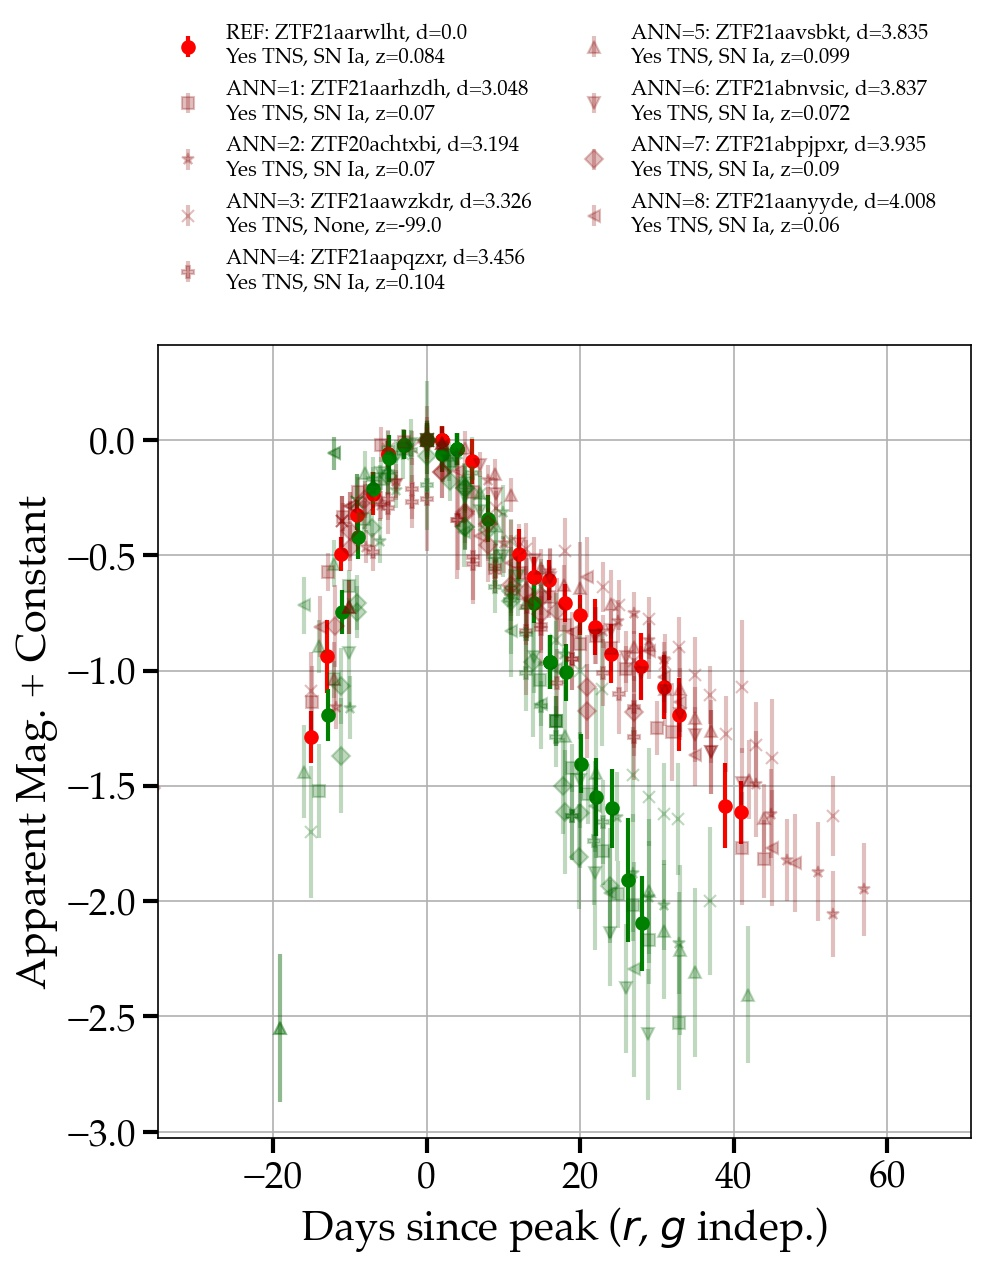
\includegraphics[width=\columnwidth]{Figures/ZTF21aarwlht_cls=SNIa_ann=8_manhattan.jpg}
    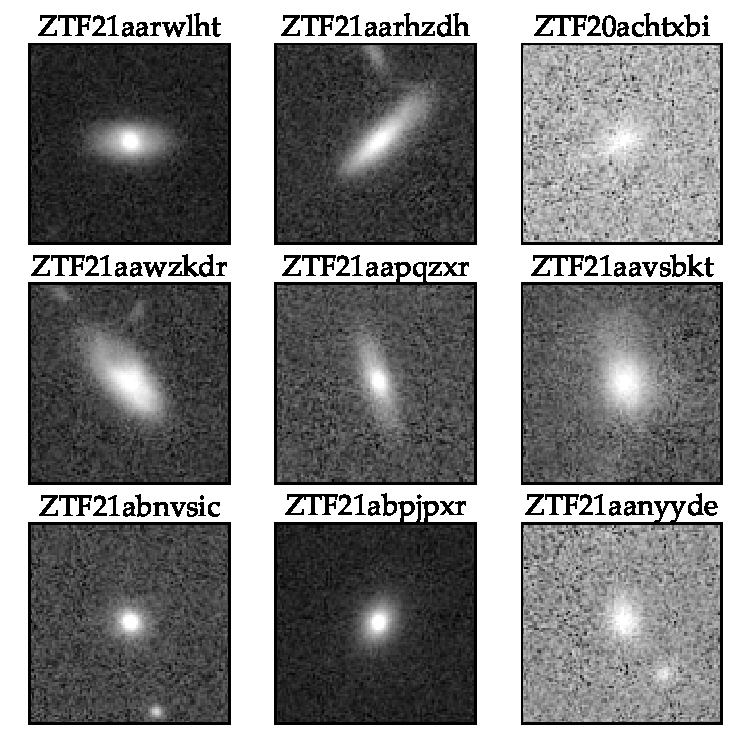
\includegraphics[width=\columnwidth]{Figures/ZTF21aarwlht_host_thumbnails_manhattan.pdf}
    \caption{
    LC+host. Manhattan. Impute missing values with median per column. No PCA. 150 trees.
    } 
    \label{fig:lc+host}
\end{figure*}
%%%%%% FIGURE %%%%%%


%%%%%%%%%%%%%%%%%%%%%%%%%%%%%%%
%%%%%%%%%%%%%%%%%%%%%%%%%%%%%%%
\subsection{Reclassification of SNe}  \label{subsec:reclass_sne}

MAKE SECTION ON RECLASSIFICATION OF SNE?
get spectra - download from yse-pz. Check of SNIax w/ that spec code (recheck absolute mags!)
	— Ref ZTF21aagqdvr/2021bfg: looks Iax 
	— ANN=1: looks Ia-norm	
	— \textbf{ANN=2 (2021fwz, ZTF21aaphlty): looks 2006gz-like (Ia-pec), at ~ -10d instead of Ia-norm}
	— ANN=3: looks Ia-norm
	— ANN=4: Ia-norm or 91T
	— ANN=5: Ia-norm
	— ANN=6: looks Ia-norm
	— ANN=7: (no spec)
	— ANN=8: looks Ia-norm (99aa)

	— Ref ZTF21abbyhvw/2021mry: Ia-pec
	— ANN=1: too noisy (but def of Ia)
	— ANN=2: too noisy (but def of Ia)
	— ANN=3: no good fit really (but def of Ia)
	— ANN=4: SLSN-II
	— ANN=5: Ia-norm
	— ANN=6: no spec
	— ANN=7: (no spec)
	— ANN=8: no spec

	— Ref ZTF21aavotzn/2021jun: Iax
	— ANN=1: looks Ia-norm
	— ANN=2: Ia-norm or 91T
	— ANN=3: noisy, can only say Ia
	— ANN=4: Ia-norm
	— ANN=5: looks Ia-norm
	— ANN=6: II
	— ANN=7: II
	— ANN=8: Ia-norm, maybe 91T

	— Ref ZTF20abwrcmq/2020sck: shit gal spectrum uploaded to TNS, too lazy to download from yse-pz. Say Iax (5 spec).
	— ANN=1: Ia-norm
	— ANN=2: Ia-norm
	— ANN=3: Ia-norm
	— ANN=4: Ic, looks marginally more Ic-BL (redward fit) to me
	— \textbf{ANN=5 (2021ars): looks Ia-91T (2007S-like) at ~-4d before peak}
	— \textbf{ANN=6 (2021ckc): looks Ia-pec, not sure what subclass, about 1 week before max light}
	— ANN=7: Ia-norm
	— ANN=8: most Ia-norm spec i’ve seen
	— ANN=9: \textbf{looks Ia-pec, a few days before peak}


 XXXXXXXXXXXXXx

 \textbf{From Ryan Foley:
both look like good candidates
“20yje almost certainly is 91bg like (you can see the Ti)
21bqg is definitely a fast decliner, but based on the spectrum, I’m not sure if I would say “91bg” - it is something of a fuzzy line though”
}
- [ ] Ref: ZTF21aawihwx (2021jvp): SN Ia-91bg-like
	— ANN=1: No spec
	— ANN=2: No spec
	— ANN=3: ZTF20acnznol (2020yje): P sure it’s 91bg-like!! Also, peak mag ~ -17.6 mag
	— ANN=4: No spec
	— ANN=5: ZTF21abcgxwy (2021nic): Ia-norm
	— ANN=6: No spec
	— ANN=7: ZTF21aaheulr (2021bja): Noisy but Ia-norm
	— ANN=8: No spec
	— ANN=9: ZTF21aagtceu (2021bqg): 91bg-like!? Also, peak mag ~ -18.1 mag



- [ ] Ref: ZTF19aaafica (2019be): SN Ia-91bg-like
	— ANN=1: No spec
	— ANN=2: ZTF21aawihwx (2021jvp): SN Ia-91bg-like
	— ANN=3: 2020abim: end of Ia?
	— ANN=4: ZTF20acnznol (2020yje): P sure it’s 91bg-like!! Also, peak mag ~ -17.6 mag
	— ANN=5: ZTF21abulrsl (2021wzb): SN Ia-91bg-like
	— ANN=6: ZTF21abcgxwy (2021nic): SN Ia-norm
	— ANN=7: ZTF21aasuego (2021inl): SN Ib-pec
	— ANN=8: No spec
	— ANN=9: ZTF21aakijia (2021csf): Ia-norm but redshift makes this under luminous peak mag ~ -18.7 mag

% %%%%%% FIGURE %%%%%%
% \begin{figure}
%     \centering
%     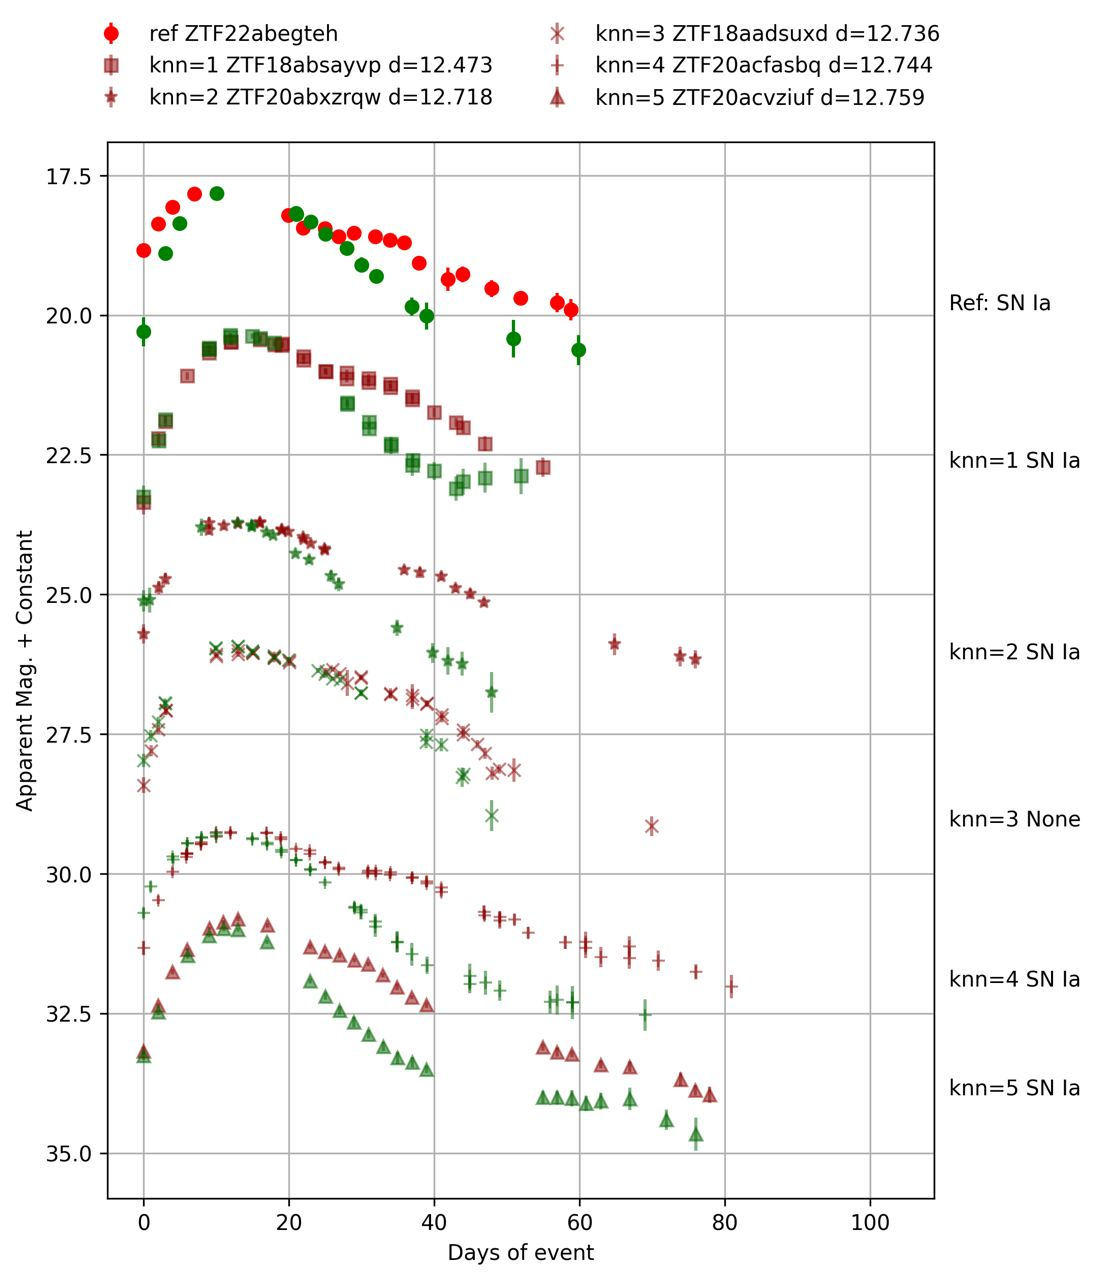
\includegraphics[width=\columnwidth]{Figures/SNIa_test.jpg}
%     \caption{
%     abc
%     } 
%     \label{fig:spec_redshift}
% \end{figure}
% %%%%%% FIGURE %%%%%%

%%%%%%%%%%%%%%%%%%%%%%%%%%%%%%%
%%%%%%%%%%%%%%%%%%%%%%%%%%%%%%%
\subsection{Unclassified Anomalies}  \label{subsec:unclass_anom}

Investigate unclassified anomalies. Some from reclassification of SNe?


%%%%%%%%%%%%%%%%%%%%%%%%%%%%%%%
%%%%%%%%%%%%%%%%%%%%%%%%%%%%%%%
\subsection{Missed Opportunity SNe}  \label{subsec:reclass_sne}

(AKA formally unreported SNe until this work).

NEED Systematic way of finding these...
    --

Distribution of missed transients as function of time/active broker teams etc. is detection and reporting efficiency getting better?



ANN=5 of https://alerce.online/object/ZTF20aatxryt: \url{https://alerce.online/object/ZTF19aaciohh} (2019baf, missed op TDE)


\url{https://alerce.online/object/ZTF21aagdrdu} (2021eik, missed op SLSN)
ANN=8 of https://alerce.online/object/ZTF20acilzkh: \url{https://alerce.online/object/ZTF21aalhtgv} (2021fao, missed op SLSN) 

 FLEET says 2021eik is not a SLSN-I, but that's just because it suggests it's a SLSN-II (which has not been tested/optimized yet)
2021fao has a P(SLSN-I) = 75\%, so, pretty good!


%%%%%%%%%%%%%%%%%%%%%%%%%%%%%%%
%%%%%%%%%%%%%%%%%%%%%%%%%%%%%%%
\section{Discussion} \label{sec:discussion}

if use feature imputation, direct values are better than PCA.

% ZTF22abvasuw/ANT2022fa0u7yowkyko (SN Ia).
% No cut on nobs (151356 dataset bank objs)
% PCA=14. 
% %%%%%% FIGURE %%%%%%
% \begin{figure*}
%     \centering
%     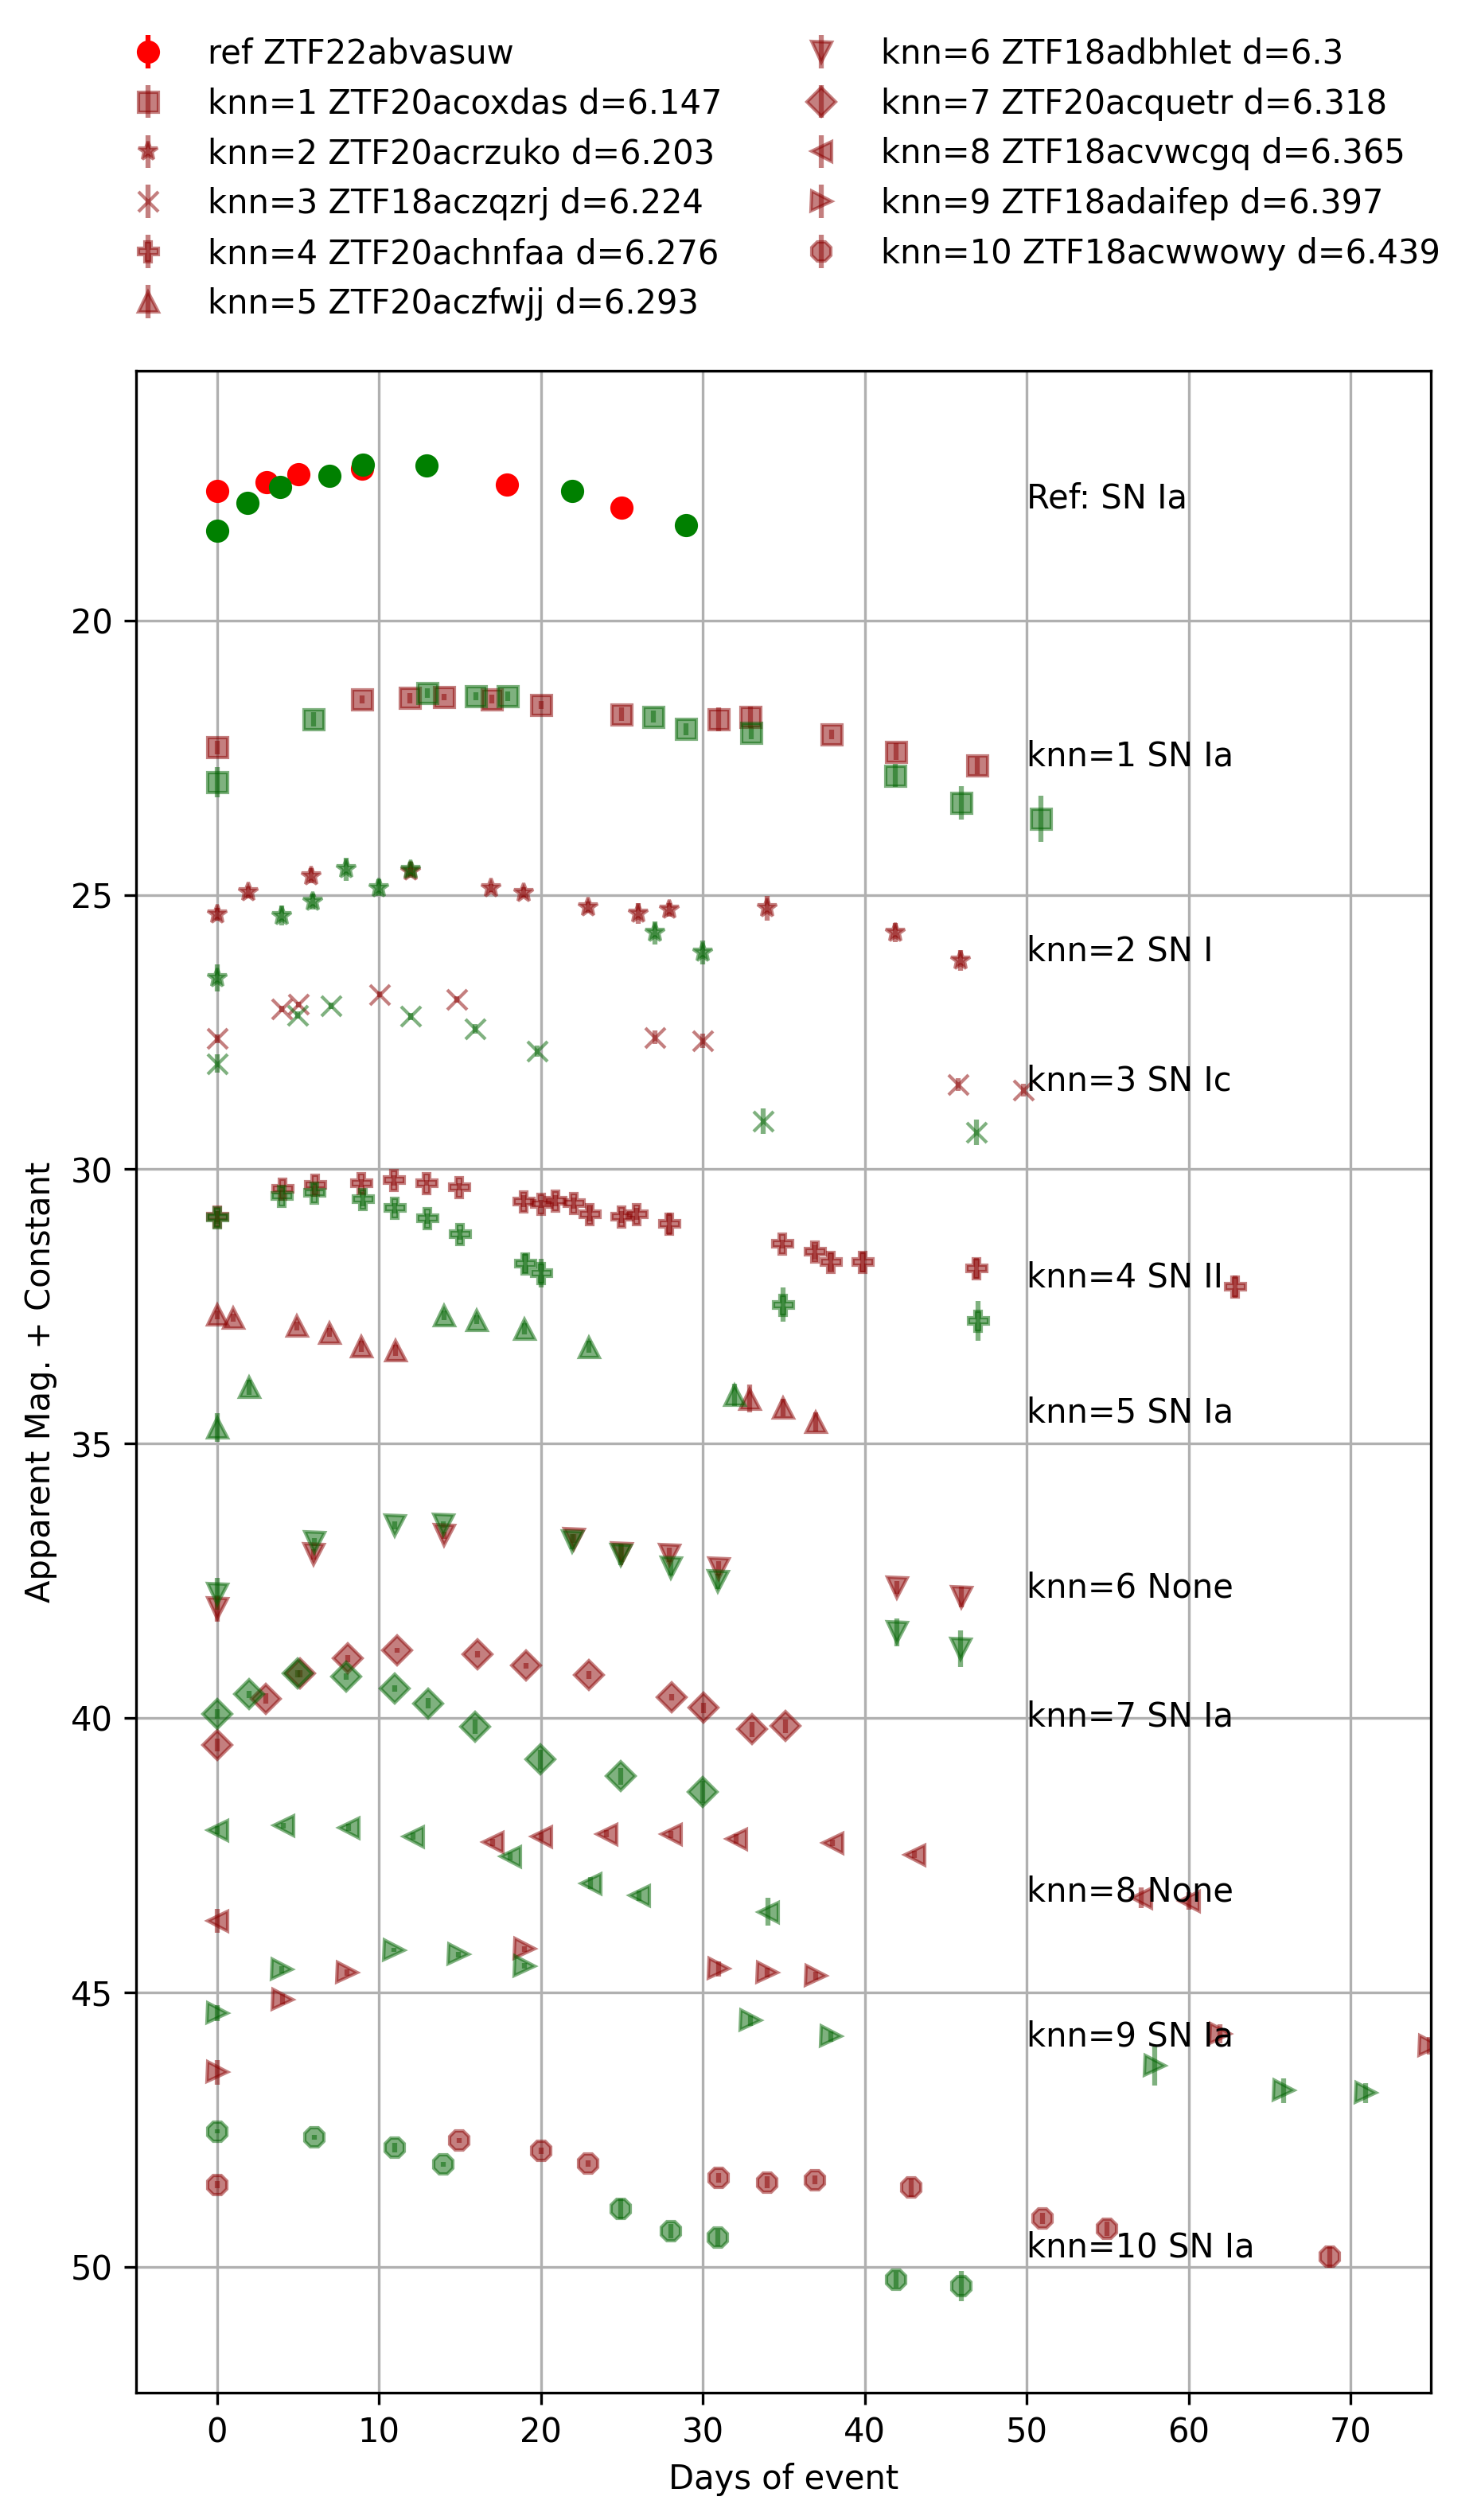
\includegraphics[width=\columnwidth]{Figures/ZTF22abvasuw_knn=10_PCA14_allobs.png}
%     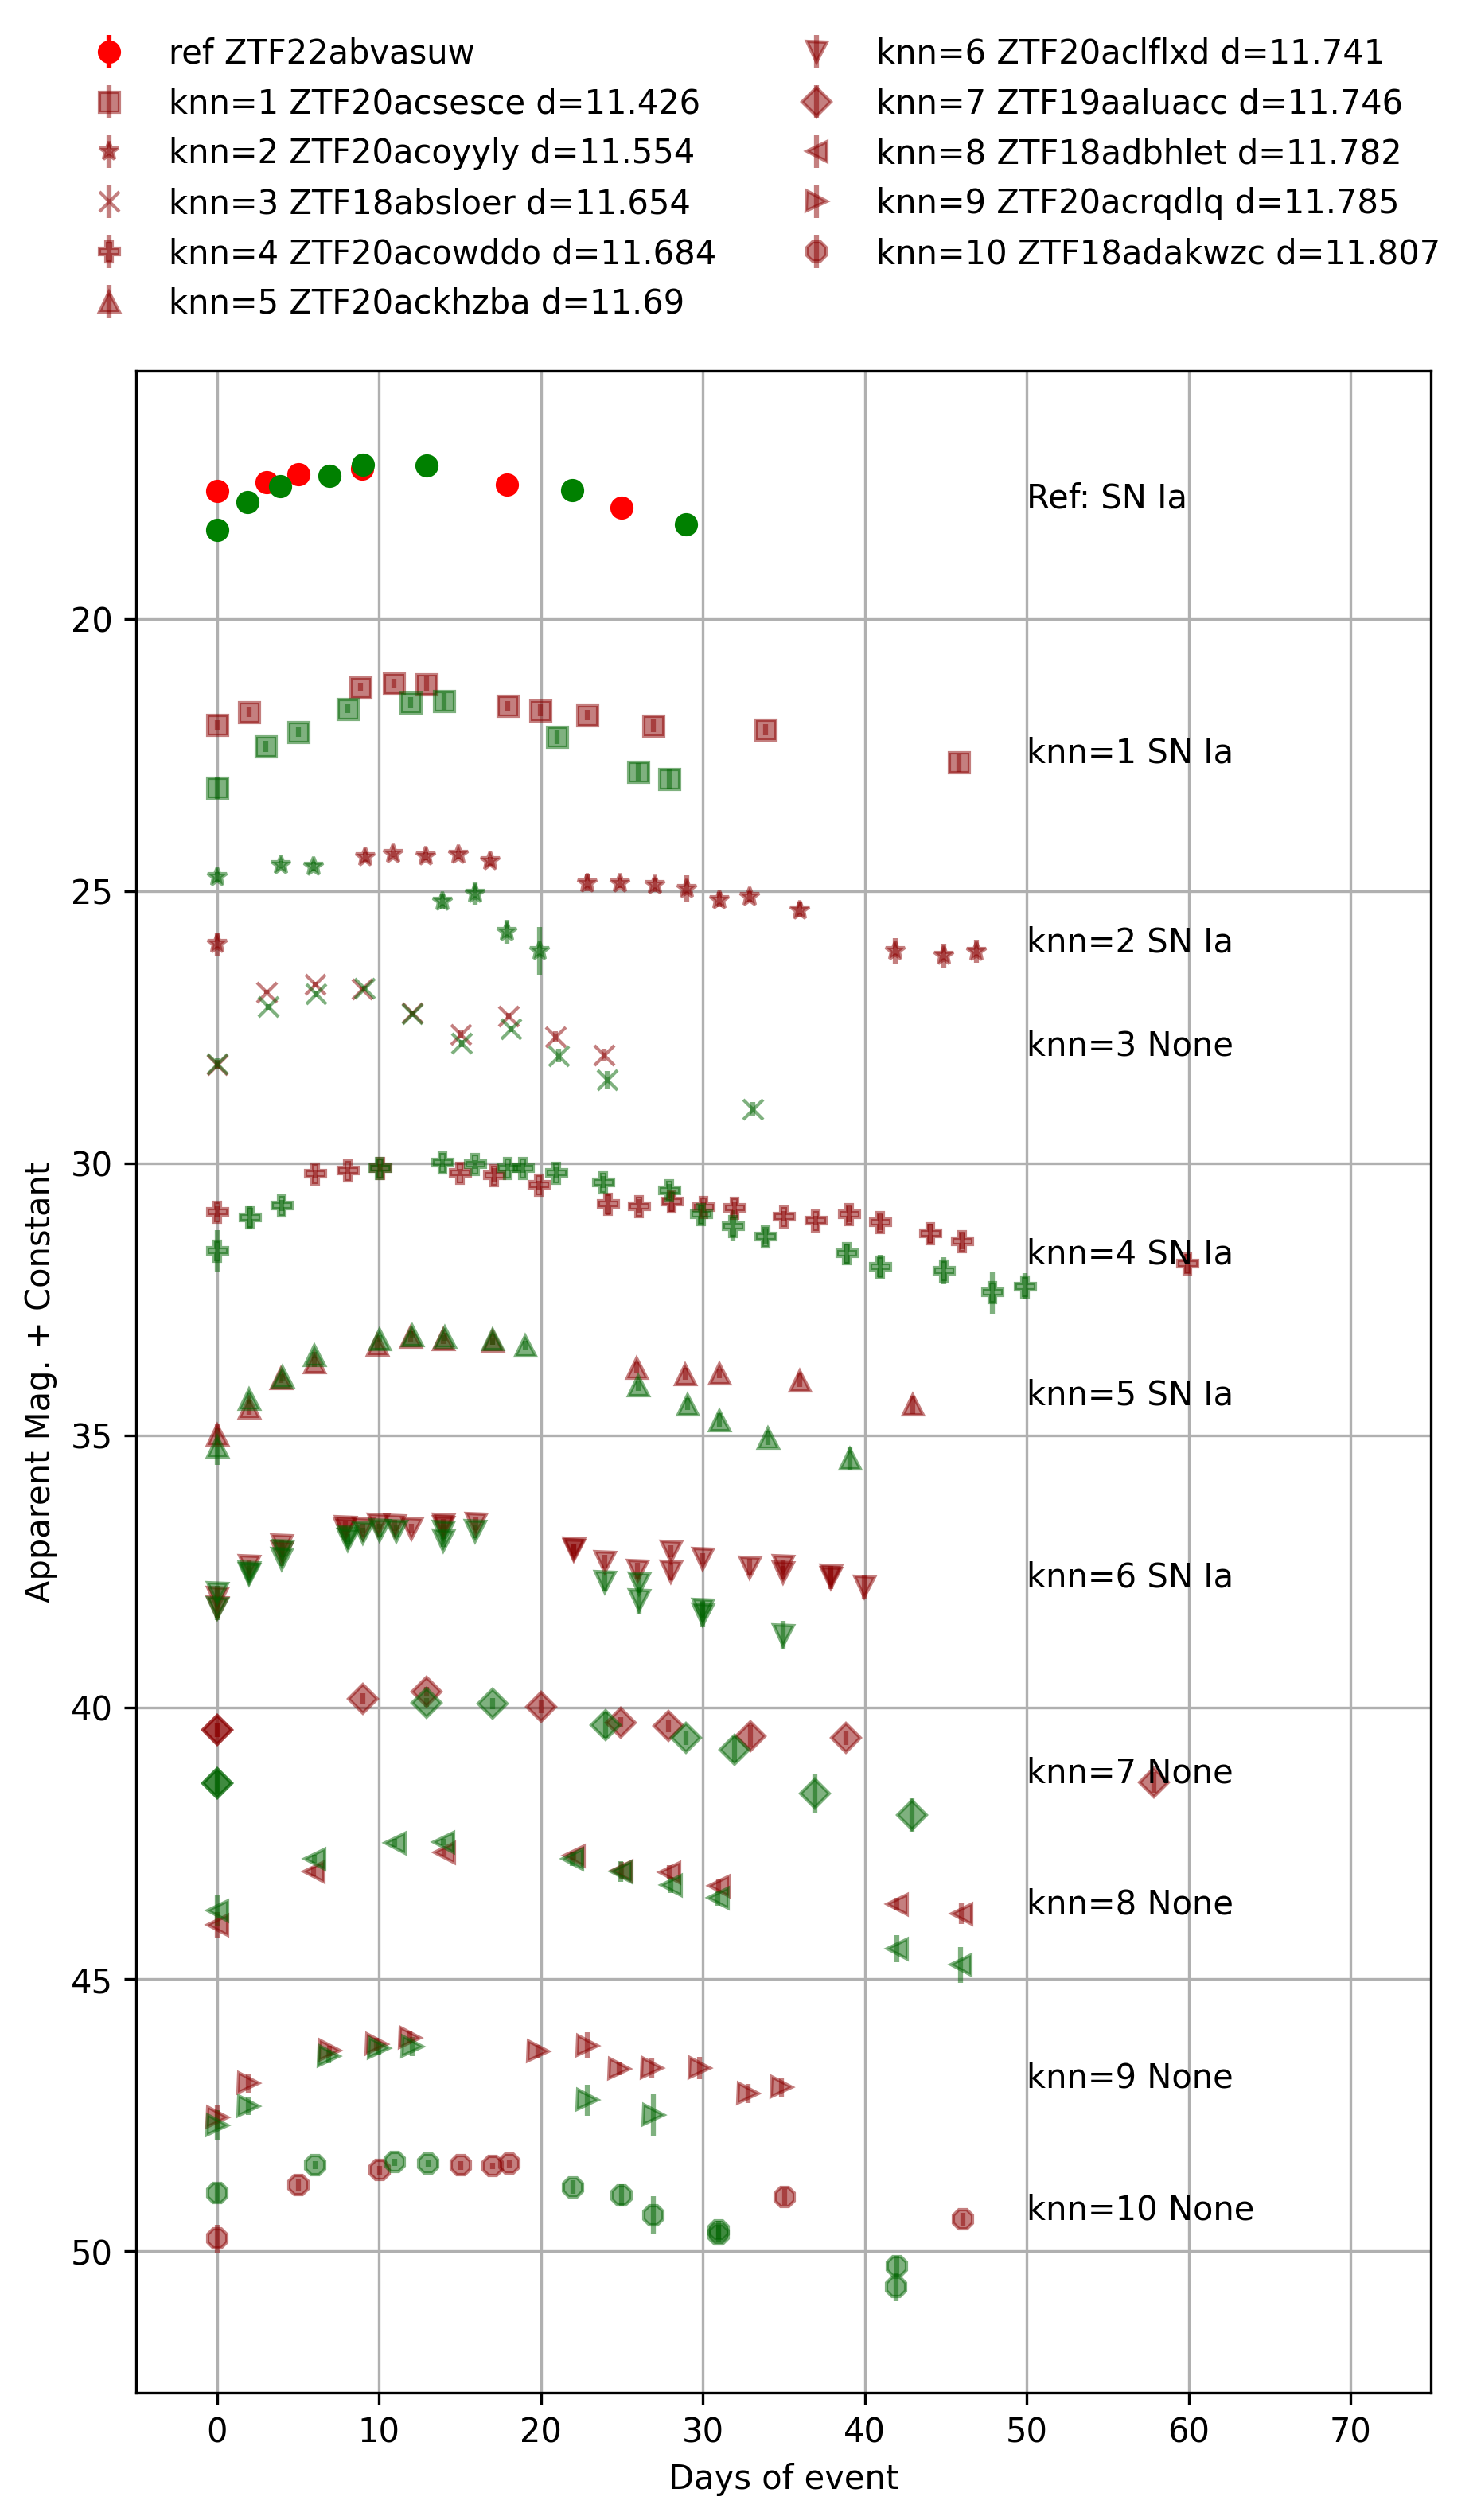
\includegraphics[width=\columnwidth]{Figures/ZTF22abvasuw_knn=10_PCA25_allobs.png}
%     \caption{
%     ZTF22abvasuw/ANT2022fa0u7yowkyko (SN Ia).
% No cut on nobs (151356 dataset bank objs).
% PCA=14 (left), PCA=25(right).
%     } 
%     \label{fig:PCA14,25allobs}
% \end{figure*}
% %%%%%% FIGURE %%%%%%

% After cut on nobs$\geq$25 (110252 dataset bank objs)
% %%%%%% FIGURE %%%%%%
% \begin{figure*}
%     \centering
%     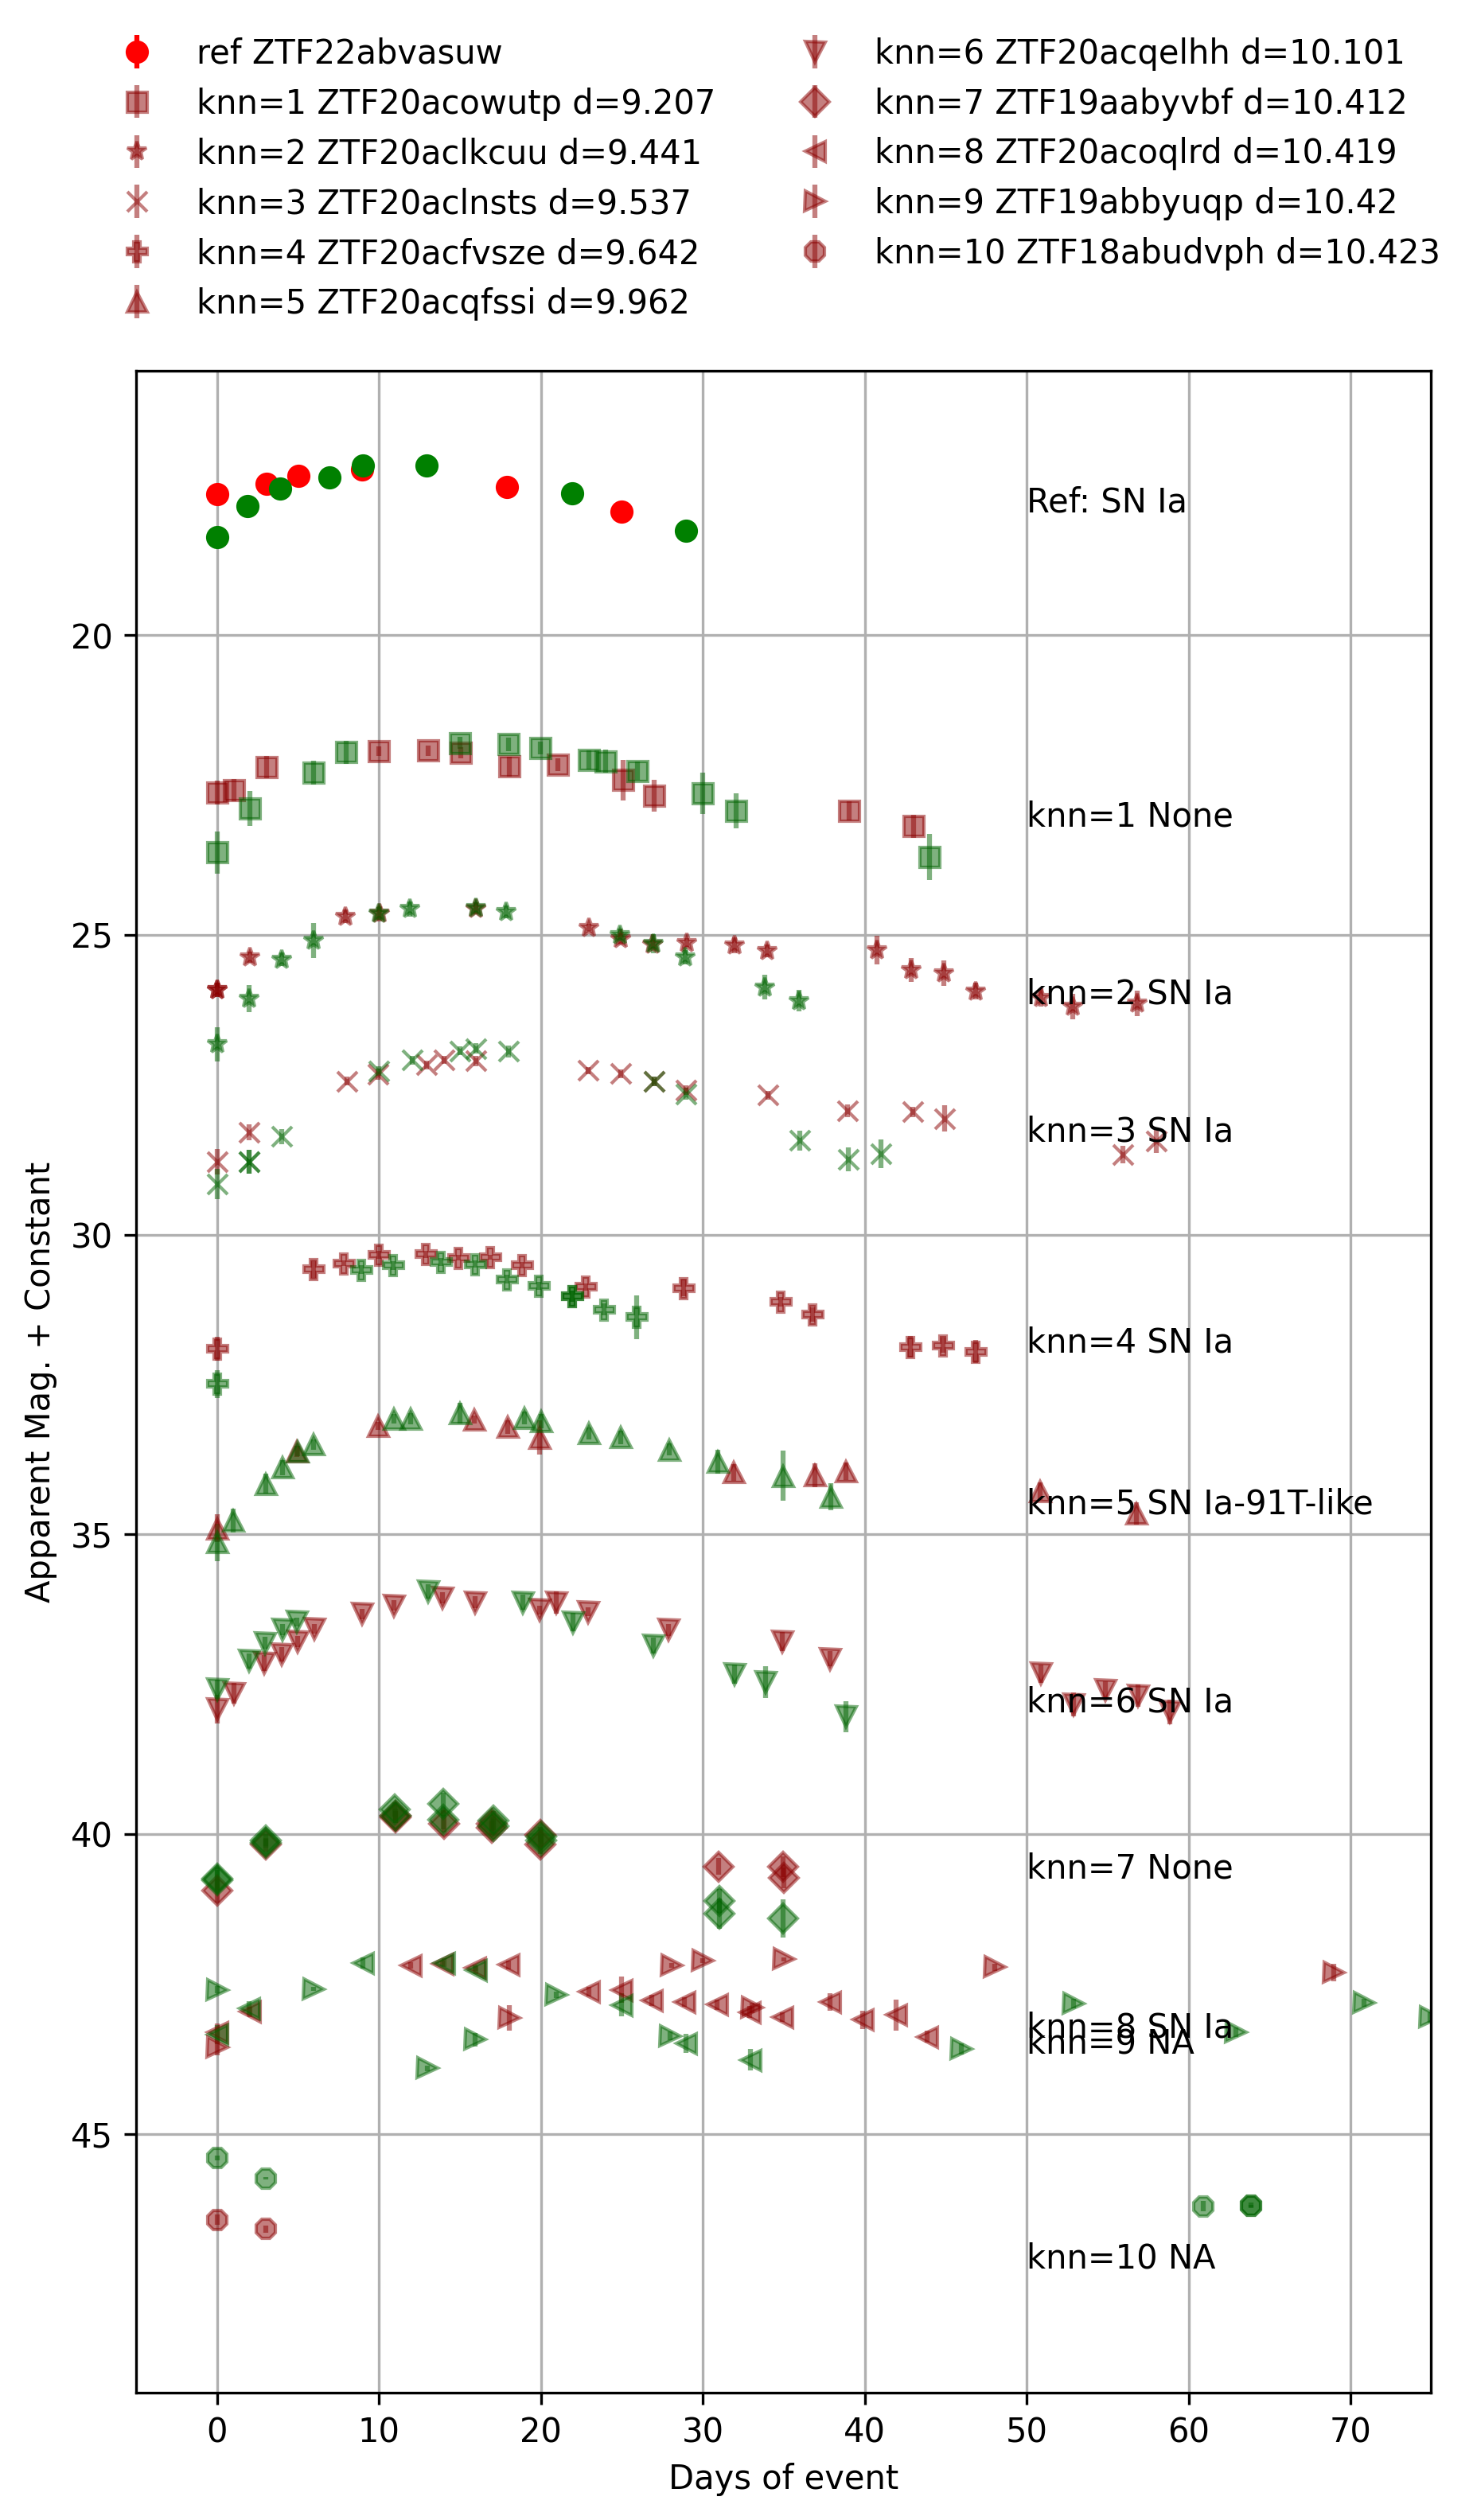
\includegraphics[width=\columnwidth]{Figures/ZTF22abvasuw_knn=10_PCA14_nobs>25.png}
%     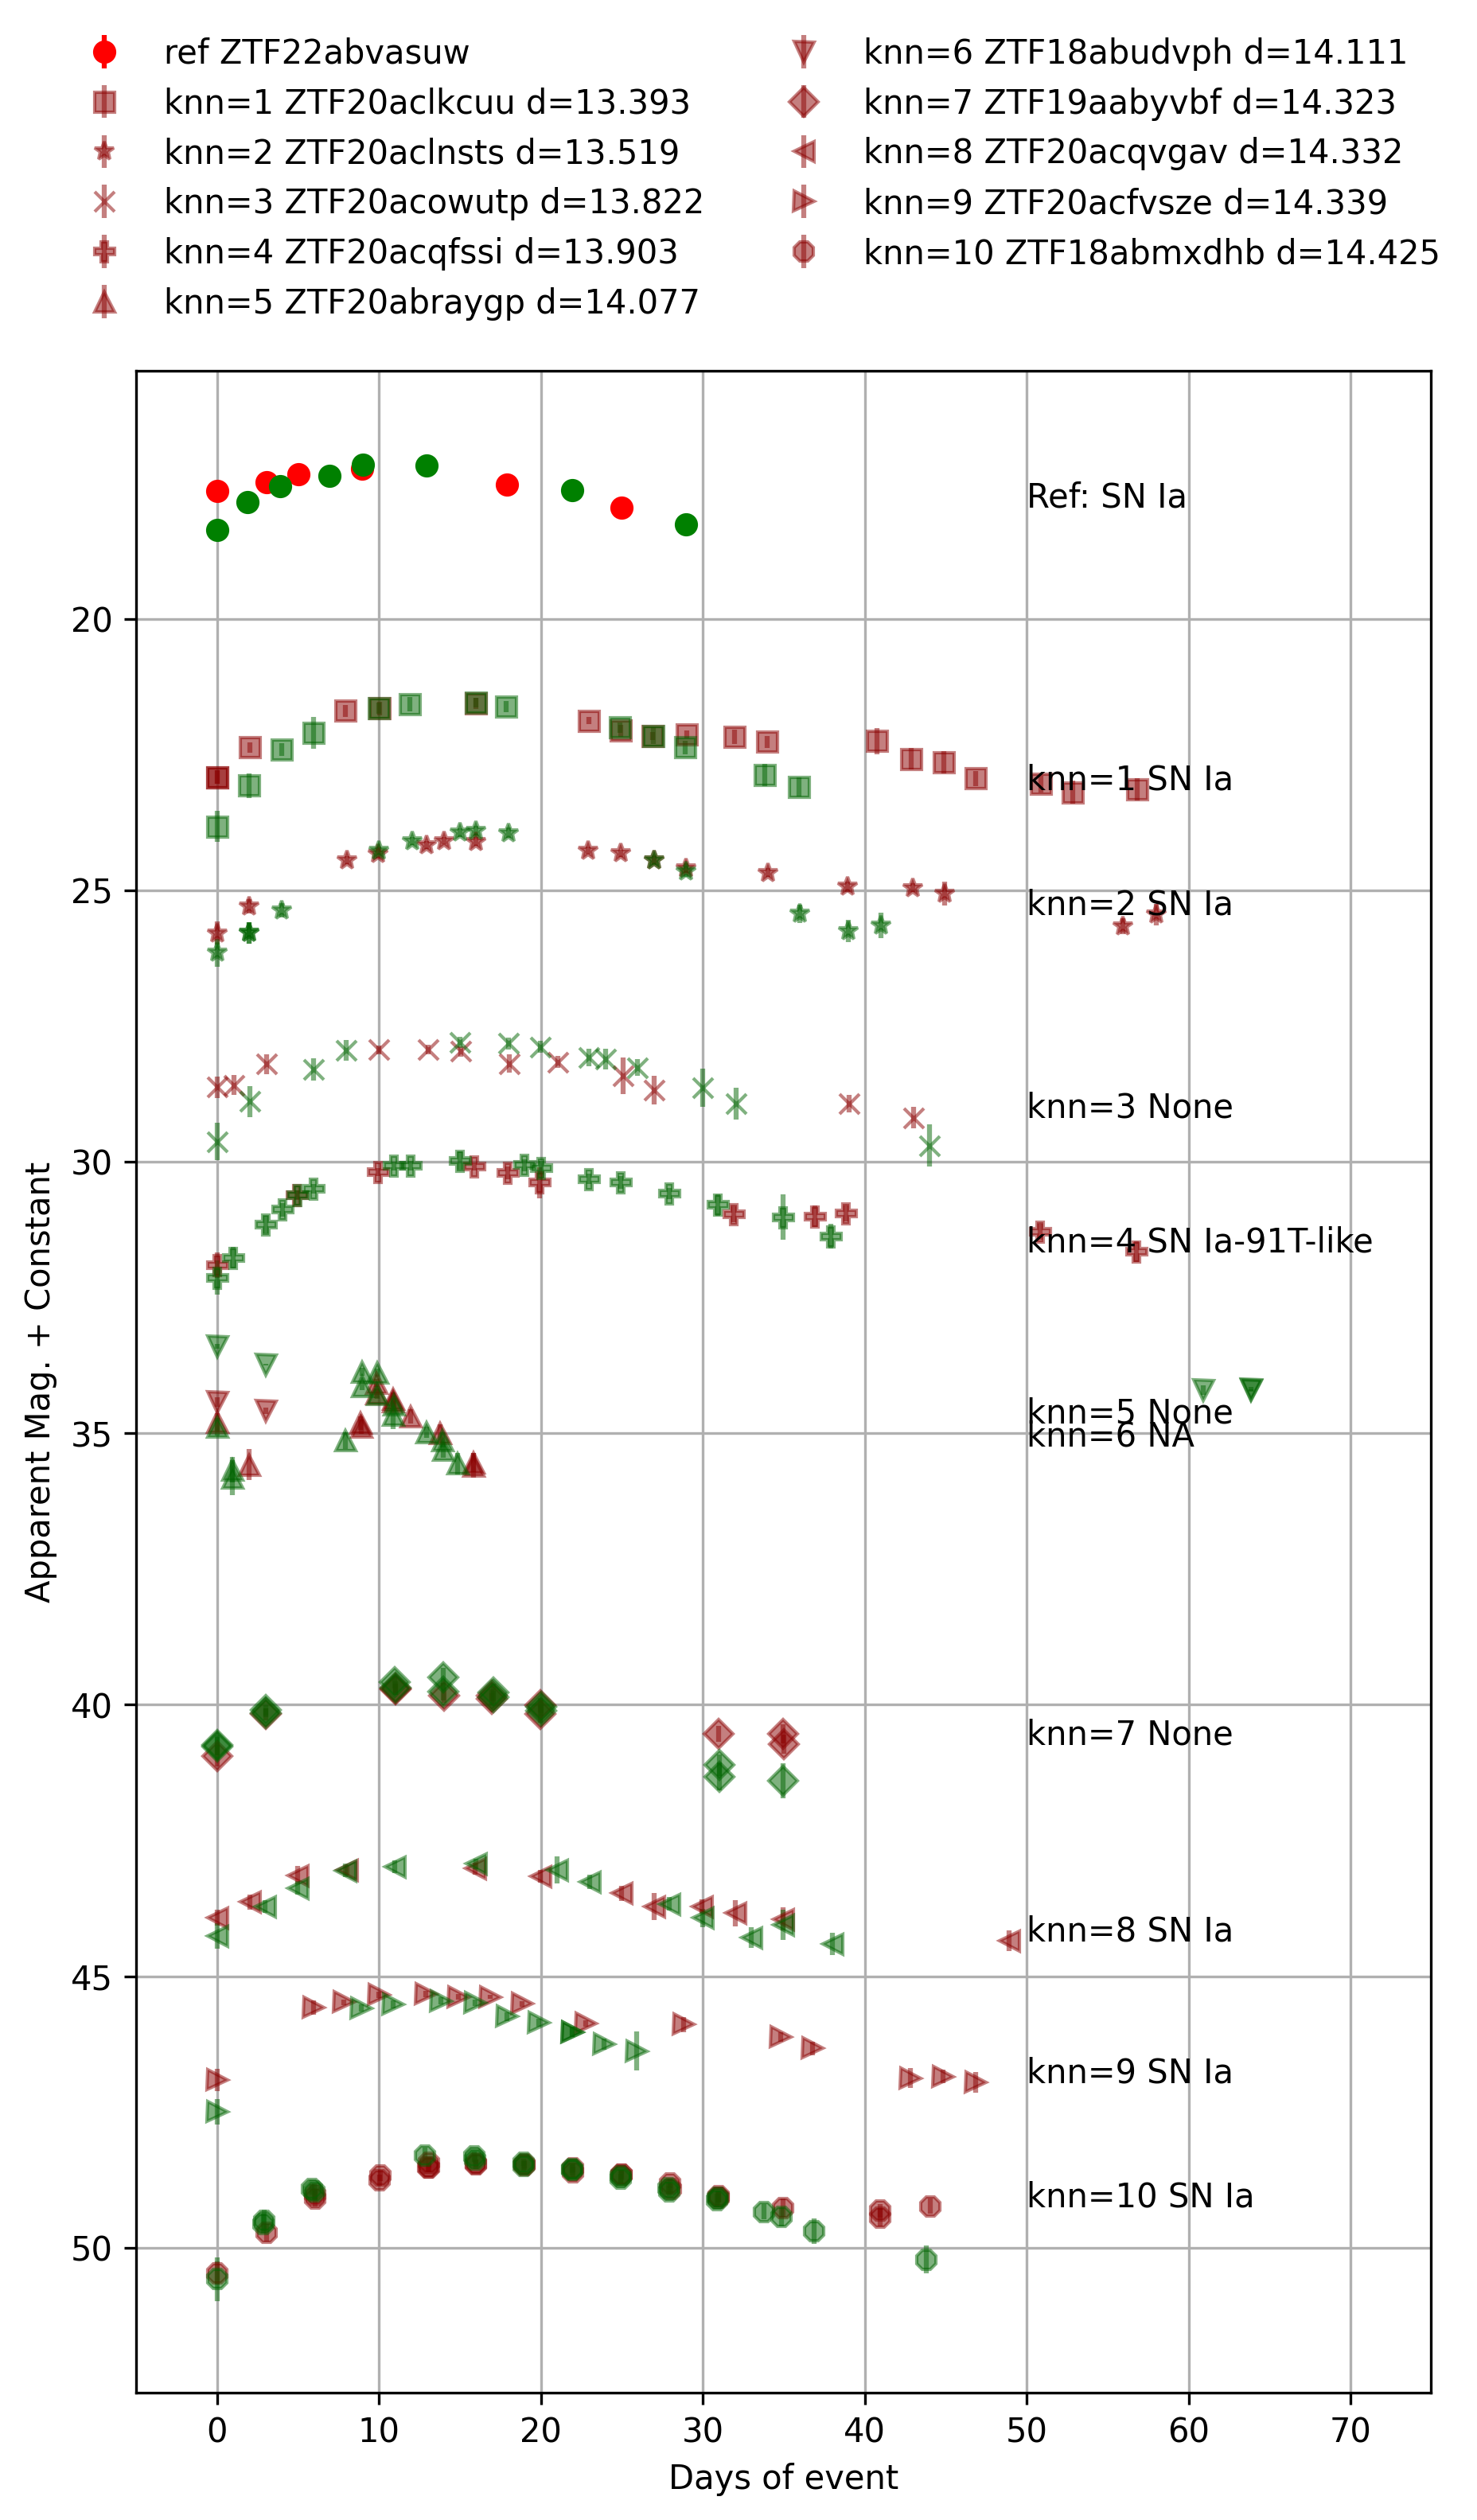
\includegraphics[width=\columnwidth]{Figures/ZTF22abvasuw_knn=10_PCA25_nobs>25.png}
%     \caption{
%     ZTF22abvasuw/ANT2022fa0u7yowkyko (SN Ia).
% After cut on nobs$\geq$25 (110252 dataset bank objs). PCA=14 (left), PCA=25(right).
%     } 
%     \label{fig:PCA14,25-nobs>25}
% \end{figure*}
% %%%%%% FIGURE %%%%%%

% After cut on nobs$\geq$40 (91926 dataset bank objs)
% %%%%%% FIGURE %%%%%%
% \begin{figure*}
%     \centering
%     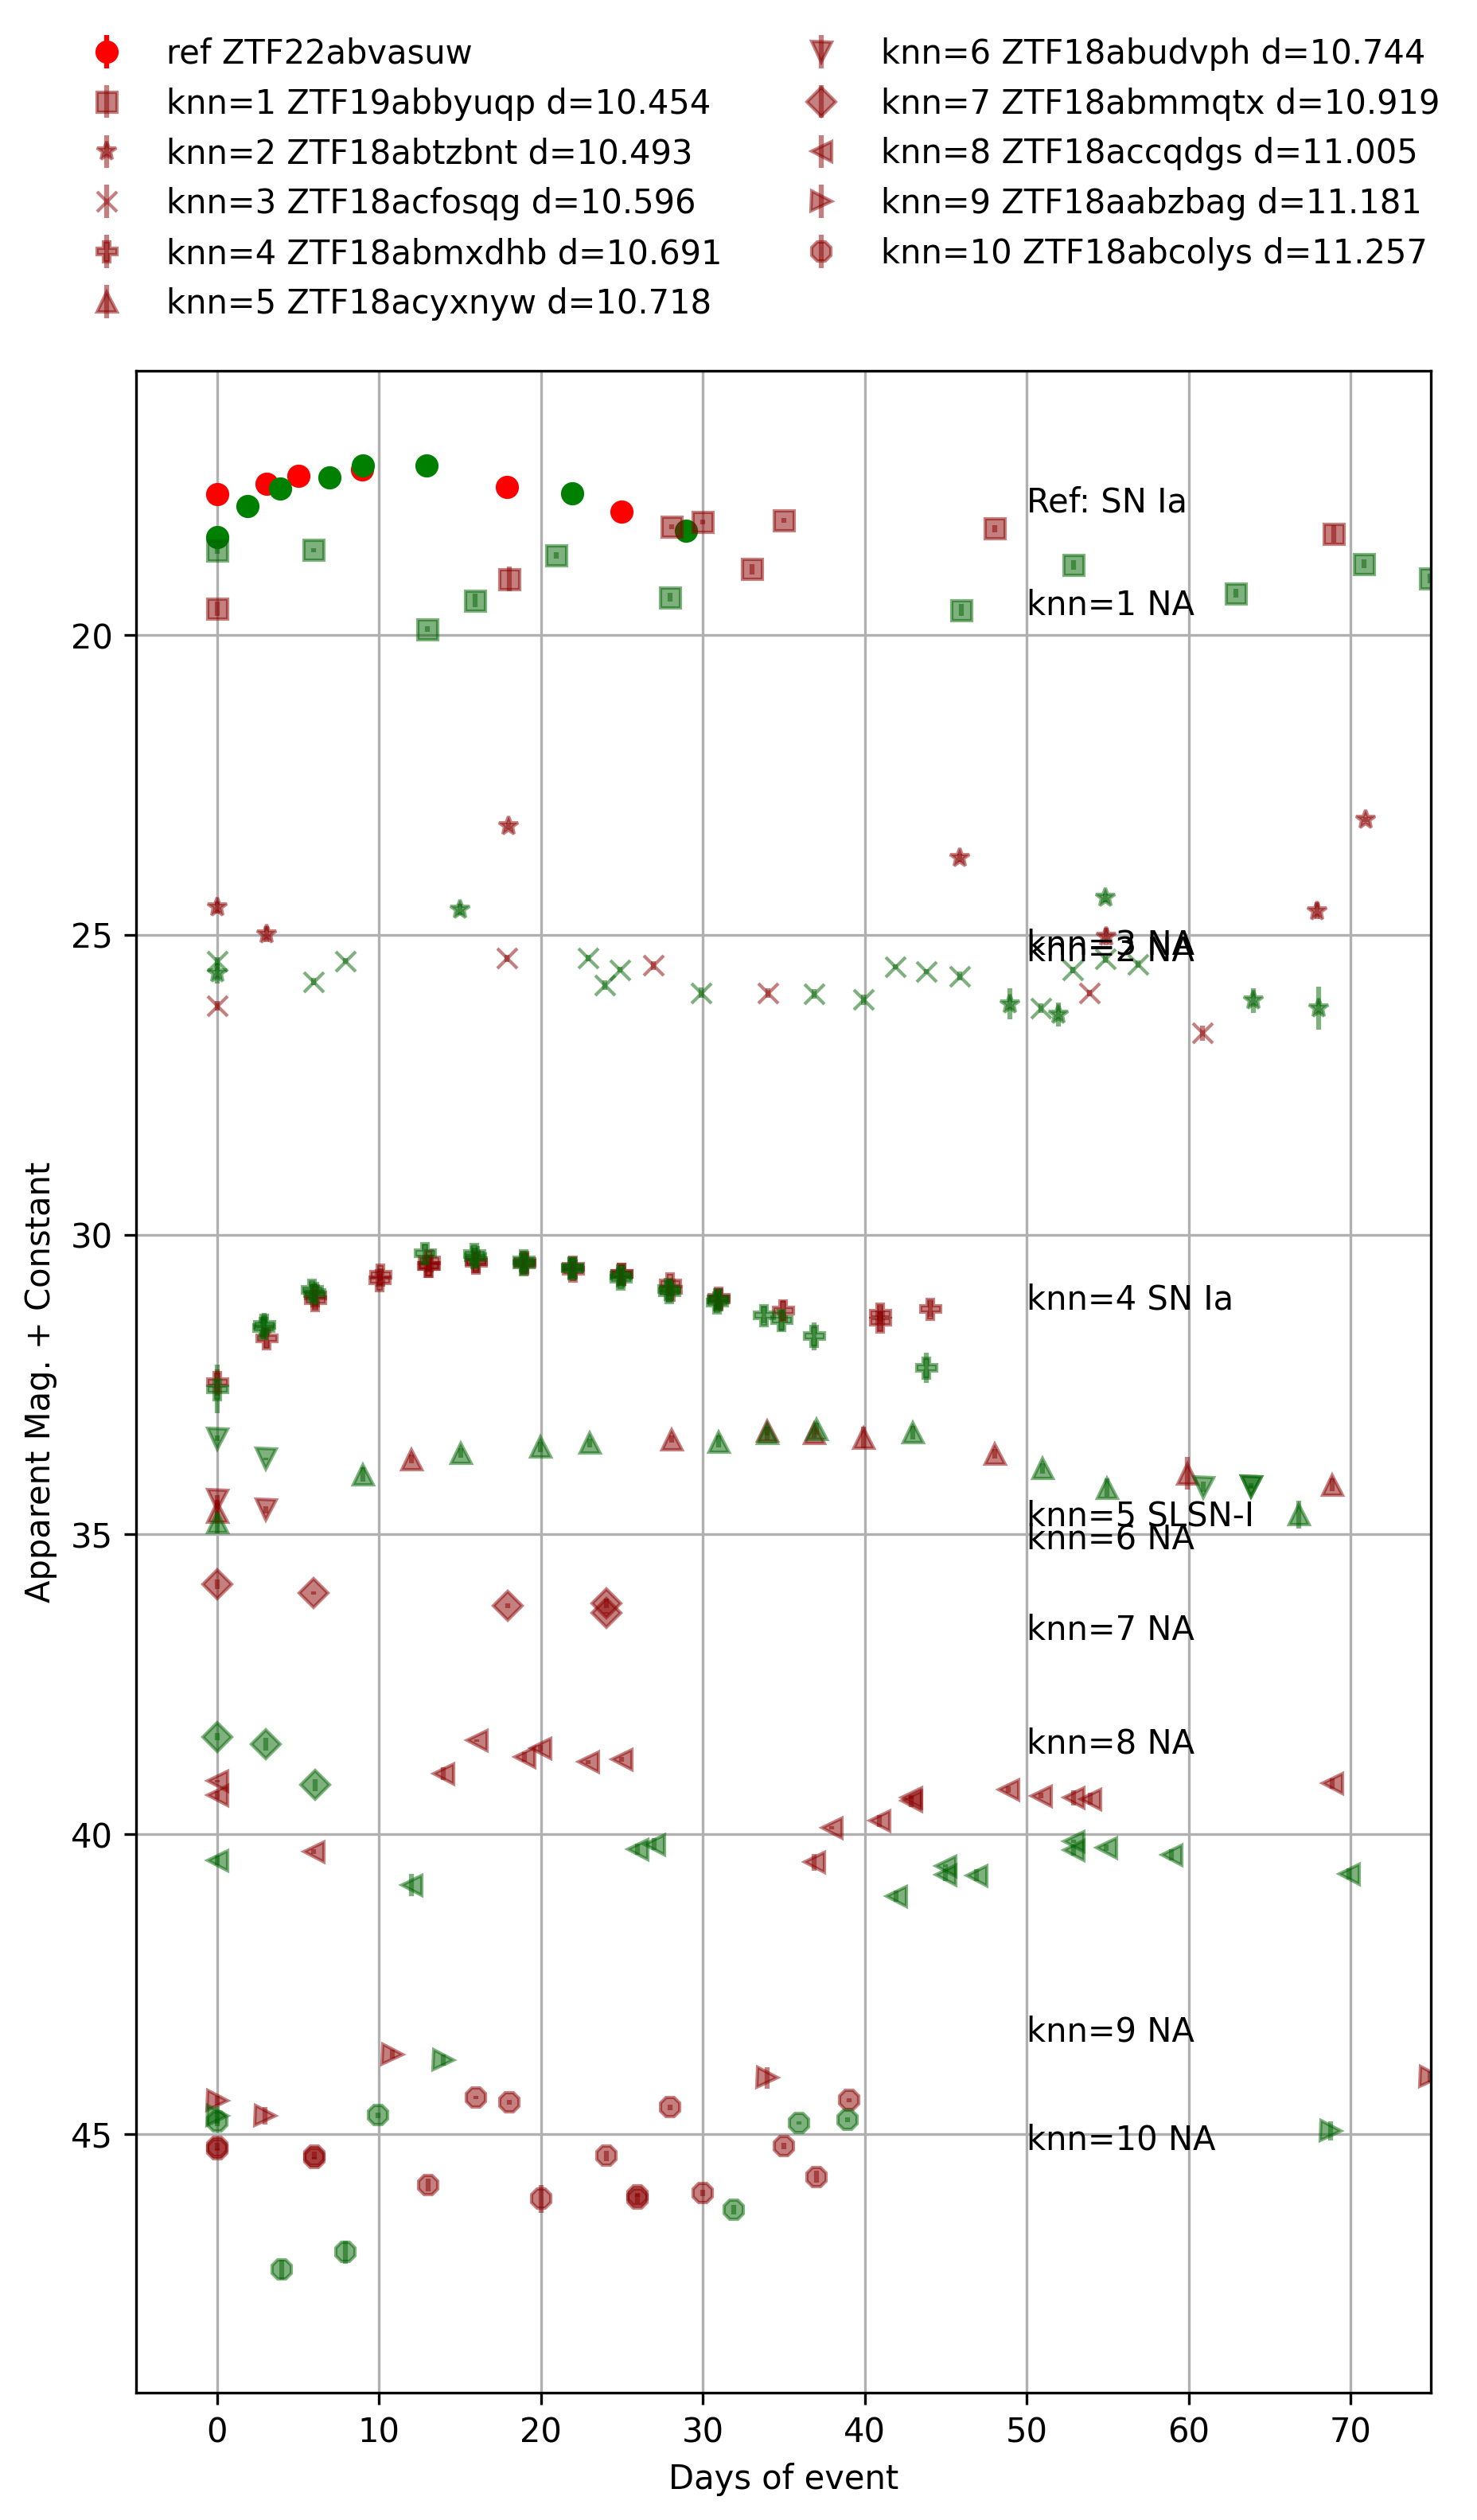
\includegraphics[width=\columnwidth]{Figures/ZTF22abvasuw_knn=10_PCA14_nobs>40.png}
%     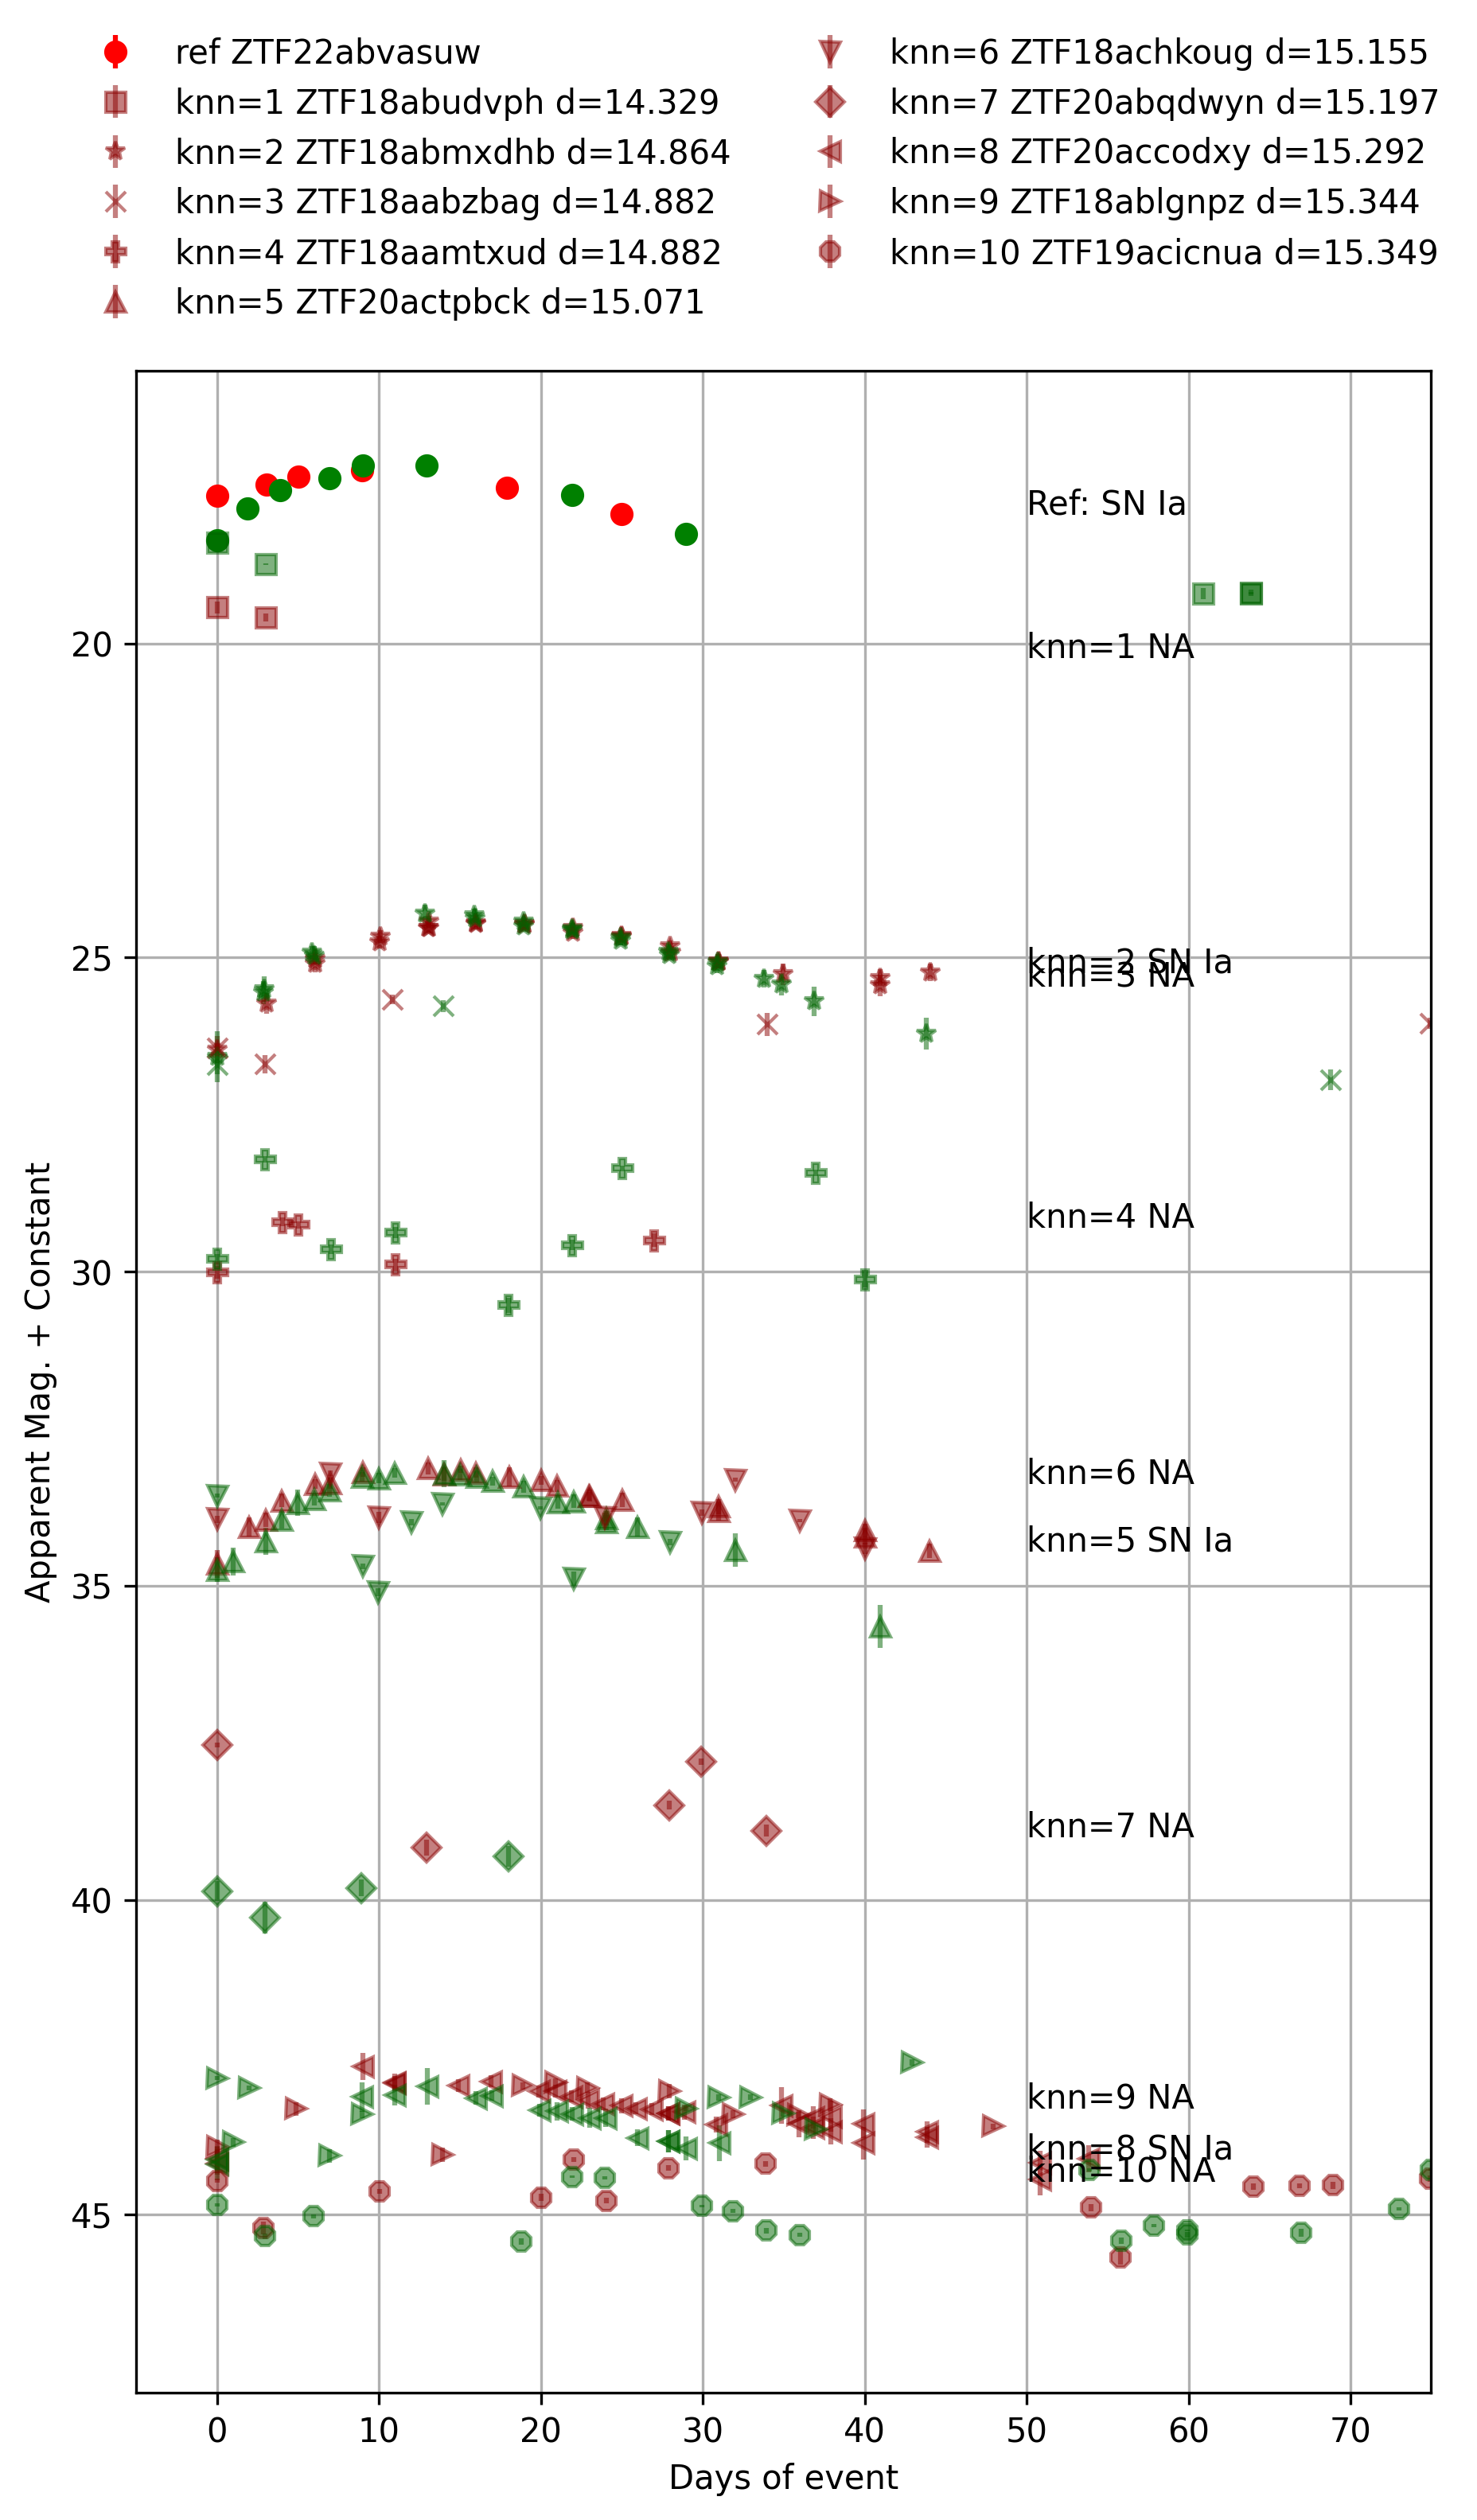
\includegraphics[width=\columnwidth]{Figures/ZTF22abvasuw_knn=10_PCA25_nobs>40.png}
%     \caption{
%     ZTF22abvasuw/ANT2022fa0u7yowkyko (SN Ia).
% After cut on nobs$\geq$40 (91926 dataset bank objs). PCA=14 (left), PCA=25(right).
%     } 
%     \label{fig:PCA14,25-nobs>40}
% \end{figure*}
% %%%%%% FIGURE %%%%%%

% \textbf{Best results are PC25, no cuts on nobs for matches! But need to retest after getting 1) updated dataset bank and 2) dataset bank to contain only variables.}

% Need to try cuts on sdss\_stars, bright\_guide\_star\_cat, gaia\_dr3\_variability, asassn\_variable\_catalog\_v2\_20190802, etc
% abc. \textbf{Overall need to get dataset bank only variables.} \par
% \textbf{ADD features that test color evolution!}


%%%%%%%%%%%%%%%%%%%%%%%%%%%%%%%
%%%%%%%%%%%%%%%%%%%%%%%%%%%%%%%
\section{Conclusion} \label{sec:conclusion}

abc\\

Our conclusions and key takeaways are as follows:
\begin{enumerate}
    \item abc
\end{enumerate}

%%%%%%%%%%%%%%%%%%%%%%%%%%%%%%%
%%%%%%%%%%%%%%%%%%%%%%%%%%%%%%%
\section{GOOD NOTES} \label{sec:notes}

- [ ] Data: streaming - Transient discovery, anomaly detection, classification(?)
    - [ ] ZTF alert stream 
        - [ ] ANTARES filters  - run on new TNS transients each night. Look at same \# KNNs
            - [ ] SNAD Miner (PCA + kdtree, or kdtree directly)
                - [ ] Find missed transients. Report to TNS
                - [ ] LC fit. Same class?
            - [ ] ANNOY (separating hyperplanes - similarity)
                - [ ] Find missed transients. Report to TNS
                - [ ] LC fit. Same class as SNe reference?
            - [ ] Overlap of algorithm results?
            - [ ] Distribution of missed transients. Timeline?
    - [ ] ELASTICC
            - [ ] SNAD Miner (PCA + kdtree, or kdtree directly)
            - [ ] ANNOY
            - [ ] Overlap of above algorithm results?
            - [ ] Same class as SNe reference? Good predictor for classification and anomaly detection?

- [ ] Some questions to answer (not exhaustive)
    - [ ] Do transients used as reference find other transients ~reliably? If so, what %?
        - [ ] Which algorithms are effective and why?
        - [ ] Are matches same/similar types? What properties do they share or not? (e.g., cadence, color evolution).
            - [ ] Is there some metric for classification (e.g. take first 10 knn with spec class, do weighted avg based on KNNs distances)
        - [ ] Can rare transients used as reference be used to find rare things?
        - [ ] Contamination of AGN and variable stars?
    - [ ] How many transients were missed in ZTF alert stream? 
        - [ ] Did this improve over time as more broker and teams used ZTF?
        - [ ] Do a LC fit to missed things.
            - [ ] What is the class distribution? 
            - [ ] Do we preferentially miss certain classes ? Faint things? at cores of galaxies?
                - [ ] How does this affect rates? e.g. How does this affect SN Ia cosmology?
        - [ ] Estimate of % things missed, and lower limit on Rubin
            - [ ] e.g. 2\%, so ~20000 SNe/yr.

            %%%%%%%%%%%%%%%%%%%%%%%%%%%%%%%
%%%%%%%%%%%%%%%%%%%%%%%%%%%%%%%

\textit{Facilities:} ZTF, ADS, TNS, NED, ATel, SNAD Viewer

\textit{Software:}
\texttt{Astropy} \citep{astropy:2013, astropy:2018}, \texttt{Matplotlib} \citep{hunter2007matplotlib}, \texttt{numpy} \citep{walt2011_numpy}, \texttt{Pandas} \citep{reback2020_pandas}, \texttt{ParSNIP} \citep{Boone2021}, \texttt{Scikit-Learn} \citep{scikit-learn}

%%%%%%%%%%%%%%%%%%%%%%%%%%%%%%%%
%%%%%%%%%%%%%%%%%%%%%%%%%%%%%%%%
\section{Acknowledgments} \label{sec:acknowledgments}

Author contributions are listed below. \\

% First Author
P.~D.~Aleo: abc \\
% Secondary Authors
K.~Malanchev: abc \\ % UPDATED!
A.~Gagliano: abc \\ % UPDATED!
G.~Narayan: abc \\ % UPDATED
YOUR NAME HERE!: abc. \\ % UPDATED

P.D.A.\ is supported by the Illinois Survey Science Graduate Fellowship from the Center for AstroPhysical Surveys (CAPS)\footnote{\url{https://caps.ncsa.illinois.edu/}} at the National Center for Supercomputing Applications (NCSA). 
A.G.\ acknowledges support from the Flatiron Institute Center for Computational Astrophysics Pre-Doctoral Fellowship Program in Spring 2022. A.G.\ is also supported by the Illinois Distinguished Fellowship, the National Science Foundation Graduate Research Fellowship Program under Grant No.\ DGE--1746047, and the Center for Astrophysical Surveys Graduate Fellowship at the University of Illinois.

Parts of this work are based on observations obtained with the Samuel Oschin Telescope 48-inch and the 60-inch Telescope at the Palomar Observatory as part of the Zwicky Transient Facility project. ZTF is supported by the National Science Foundation under Grants No.\ AST--1440341 and AST--2034437 and a collaboration including current partners Caltech, IPAC, the Weizmann Institute of Science, the Oskar Klein Center at Stockholm University, the University of Maryland, Deutsches Elektronen-Synchrotron and Humboldt University, the TANGO Consortium of Taiwan, the University of Wisconsin at Milwaukee, Trinity College Dublin, Lawrence Livermore National Laboratories, IN2P3, University of Warwick, Ruhr University Bochum, Northwestern University and former partners the University of Washington, Los Alamos National Laboratories, and Lawrence Berkeley National Laboratories. Operations are conducted by COO, IPAC, and UW.
The ZTF forced-photometry service was funded under the Heising-Simons Foundation grant \#12540303 (PI: Graham). 

abc!

%% For this sample we use BibTeX plus aasjournals.bst to generate the
%% the bibliography. The sample63.bib file was populated from ADS. To
%% get the citations to show in the compiled file do the following:
%%
%% pdflatex sample63.tex
%% bibtext sample63
%% pdflatex sample63.tex
%% pdflatex sample63.tex

\bibliography{references}{}
\bibliographystyle{aasjournal}

\appendix

%\section{Supplementary Materials} 
%\label{sec:appendix}

%%%%%%%%%%%%%%%%%%%%%%%%%%%%%%
%%%%%%%%%%%%%%%%%%%%%%%%%%%%%%
\section{Light Curve Features}
\label{appx:lc_features}


\counterwithin{figure}{section}
\counterwithin{table}{section}
\renewcommand{\thefigure}{A.\arabic{figure}}
\setcounter{figure}{0}
\renewcommand{\thetable}{A.\arabic{table}} \setcounter{table}{0}

%%%%%%%%%%%%%%%%%%%%%%%%%%%%%%
% Put in Appendix
% LC features from lc_feature_extractor (light-curve package version 0.2.2): 
% https://docs.rs/light-curve-feature/0.2.2/light_curve_feature/features/index.html
Our light curve features are extracted with the \texttt{lc\_feature\_extractor} filter in ANTARES using the \texttt{light-curve} package. We extract the same features for $r$ and $g$ band, comprising 62 total features (31 $r$ band, 31 $g$ band). A brief description of each feature is as follows:

\begin{itemize}
    \item \texttt{feature\_amplitude\_magn}: Half amplitude of magnitude \citep{Malanchev2021}.
    \item \texttt{feature\_anderson\_darling\_normal\_magn}: Unbiased Anderson–Darling normality test statistic for magnitude \citep{Malanchev2021}.
    \item \texttt{feature\_beyond\_1\_std\_magn}: Fraction of observations beyond $n=1 \sigma_{m}$ from the mean magnitude $\langle m \rangle$ \citep{D'Isanto2016}.
    \item \texttt{feature\_beyond\_2\_std\_magn}: Fraction of observations beyond $n=2 \sigma_{m}$ from the mean magnitude $\langle m \rangle$ \citep{D'Isanto2016}.
    \item \texttt{feature\_cusum\_magn}: A range of cumulative sums dependent on the number of observations, mean magnitude, and magnitude standard deviation \citep{Kim2014}.
    \item \texttt{feature\_inter\_percentile\_range\_2\_magn}: Inter-percentile range for $p=0.02$, where $p$ is the pth quantile of the magnitude distribution \citep{Malanchev2021}.
    \item \texttt{feature\_inter\_percentile\_range\_10\_magn}: Inter-percentile range for $p=0.10$, where $p$ is the pth quantile of the magnitude distribution. A special case of the interpercetile range known as the interdecile range \citep{Malanchev2021}.
    \item \texttt{feature\_inter\_percentile\_range\_25\_magn}: Inter-percentile range for $p=0.25$, where $p$ is the pth quantile of the magnitude distribution. A special case of the interpercetile range known as the interquartile range\citep{Malanchev2021}.
    \item \texttt{feature\_kurtosis\_magn}: Excess kurtosis of magnitude \citep{Malanchev2021}.
    \item \texttt{feature\_linear\_fit\_slope\_magn}: The slope of the light curve in the least squares fit of the linear stochastic model with Gaussian noise described by observation errors \{$\delta_{i}$\} \citep{Malanchev2021}.
    \item \texttt{feature\_linear\_fit\_slope\_sigma\_magn}: The error of the slope of the light curve in the least squares fit of the linear stochastic model with Gaussian noise described by observation errors \{$\delta_{i}$\} \citep{Malanchev2021}.
    \item \texttt{feature\_magnitude\_percentage\_ratio\_40\_5\_magn}: The magnitude 40 to 5 ratio, written in terms of the magnitude distribution quantile function $Q$. \citep{D'Isanto2016}.
    \item \texttt{feature\_magnitude\_percentage\_ratio\_20\_5\_magn}: The magnitude 20 to 5 ratio, written in terms of the magnitude distribution quantile function $Q$. \citep{D'Isanto2016}.
    \item \texttt{feature\_mean\_magn}: The non-weighted mean magnitude.
    \item \texttt{feature\_median\_absolute\_deviation\_magn}: The median of the absolute value of the difference between magnitude and its median \citep{D'Isanto2016}.
    \item \texttt{feature\_percent\_amplitude\_magn}: The maximum deviation of magnitude from its median \citep{D'Isanto2016}.
    \item \texttt{feature\_median\_buffer\_range\_percentage\_10\_magn}: The fraction of observations inside Median($m$) $\pm 10 \times$ (max($m$)-min($m$))/2 interval \citep{D'Isanto2016}.
    \item \texttt{feature\_median\_buffer\_range\_percentage\_20\_magn}: The fraction of observations inside Median($m$) $\pm 20 \times$ (max($m$)-min($m$))/2 interval \citep{D'Isanto2016}.
    \item \texttt{feature\_percent\_difference\_magnitude\_percentile\_5\_magn}: Ratio of $p$=5th inter-percentile range to the median \citep{Malanchev2021}.
    \item \texttt{feature\_percent\_difference\_magnitude\_percentile\_10\_magn}: Ratio of $p$=10th inter-percentile range to the median \citep{Malanchev2021}.
    \item \texttt{feature\_skew\_magn}: Skewness of magnitude, $G_{1}$ \citep{Malanchev2021}.
    \item \texttt{feature\_standard\_deviation\_magn}: 	Standard deviation of magnitude, $\sigma_{m}$ \citep{Malanchev2021}.
    \item \texttt{feature\_stetson\_k\_magn}: Stetson $K$ coefficient described light curve shape of magnitude \citep{Stetson1996}.
    \item \texttt{feature\_weighted\_mean\_magn}: Weighted mean magnitude \citep{Malanchev2021}.
    \item \texttt{feature\_anderson\_darling\_normal\_flux}: Unbiased Anderson–Darling normality test statistic for flux \citep{Malanchev2021}.
    \item \texttt{feature\_cusum\_flux}: A range of cumulative sums dependent on the number of observations, mean flux, and flux standard deviation \citep{Kim2014}.
    \item \texttt{feature\_excess\_variance\_flux}: Measure of the flux variability amplitude \citep{Sanchez2017}.
    \item \texttt{feature\_kurtosis\_flux}: Excess kurtosis of flux \citep{Malanchev2021}.
    \item \texttt{feature\_mean\_variance\_flux}: Standard deviation of flux to mean flux ratio \citep{Malanchev2021}.
    \item \texttt{feature\_skew\_flux}: Skewness of flux \citep{Malanchev2021}.
    \item \texttt{feature\_stetson\_k\_flux}: Stetson $K$ coefficient described light curve shape of flux \citep{Stetson1996}.
\end{itemize}


The full documentation, including equations, can be found here: \url{https://docs.rs/light-curve-feature/0.2.2/light_curve_feature/features/index.html}.


%%%%%%%%%%%%%%%%%%%%%%%%%%%%%%
%%%%%%%%%%%%%%%%%%%%%%%%%%%%%%
\section{Host Galaxy Features}
\label{appx:host_gal_features}


\counterwithin{figure}{section}
\counterwithin{table}{section}
\renewcommand{\thefigure}{A.\arabic{figure}}
\setcounter{figure}{0}
\renewcommand{\thetable}{A.\arabic{table}} \setcounter{table}{0}

%%%%%%%%%%%%%%%%%%%%%%%%%%%%%%
% Put in Appendix
% ps1 features: https://outerspace.stsci.edu/display/PANSTARRS/PS1+Database+object+and+detection+tables 
Our host galaxy features and a brief description are as follows:

\begin{itemize}
    \item \texttt{gmomentXX}: Second moment $M_{xx}$ for $g$ filter stack detection. 
    \item \texttt{gmomentXY}: Second moment $M_{xy}$ for $g$ filter stack detection. 
    \item \texttt{gmomentYY}: Second moment $M_{yy}$ for $g$ filter stack detection. 
    \item \texttt{gmomentR1}: First radial moment for $g$ filter stack detection.
    \item \texttt{gmomentRH}: Half radial moment ($r^{0.5}$ weighting) for $g$ filter stack detection.
    \item \texttt{gPSFFlux}: PSF flux from $g$ filter stack detection.
    \item \texttt{gApFlux}: Aperture flux from $g$ filter stack detection.
    \item \texttt{gKronFlux}: \cite{Kron1980} flux from $g$ filter stack detection.
    \item \texttt{gKronRad}: \cite{Kron1980} radius from $g$ filter stack detection.
    \item \texttt{gExtNSigma}: An extendedness measure for the $g$ filter stack detection based on the deviation between PSF and \cite{Kron1980} magnitudes, normalized by the PSF magnitude uncertainty.
    \item \texttt{rmomentXX}: Second moment $M_{xx}$ for $r$ filter stack detection. 
    \item \texttt{rmomentXY}: Second moment $M_{xy}$ for $r$ filter stack detection. 
    \item \texttt{rmomentYY}: Second moment $M_{yy}$ for $r$ filter stack detection. 
    \item \texttt{rmomentR1}: First radial moment for $r$ filter stack detection.
    \item \texttt{rmomentRH}: Half radial moment ($r^{0.5}$ weighting) for $r$ filter stack detection.
    \item \texttt{rPSFFlux}: PSF flux from $r$ filter stack detection.
    \item \texttt{rApFlux}: Aperture flux from $r$ filter stack detection.
    \item \texttt{rKronFlux}: \cite{Kron1980} flux from $r$ filter stack detection.
    \item \texttt{rKronRad}: \cite{Kron1980} radius from $r$ filter stack detection.
    \item \texttt{rExtNSigma}: An extendedness measure for the $r$ filter stack detection based on the deviation between PSF and \cite{Kron1980} magnitudes, normalized by the PSF magnitude uncertainty.
    \item \texttt{imomentXX}: Second moment $M_{xx}$ for $i$ filter stack detection. 
    \item \texttt{imomentXY}: Second moment $M_{xy}$ for $i$ filter stack detection. 
    \item \texttt{imomentYY}: Second moment $M_{yy}$ for $i$ filter stack detection. 
    \item \texttt{imomentR1}: First radial moment for $i$ filter stack detection.
    \item \texttt{imomentRH}: Half radial moment ($r^{0.5}$ weighting) for $i$ filter stack detection.
    \item \texttt{iPSFFlux}: PSF flux from $i$ filter stack detection.
    \item \texttt{iApFlux}: Aperture flux from $i$ filter stack detection.
    \item \texttt{iKronFlux}: \cite{Kron1980} flux from $i$ filter stack detection.
    \item \texttt{iKronRad}: \cite{Kron1980} radius from $i$ filter stack detection.
    \item \texttt{iExtNSigma}: An extendedness measure for the $i$ filter stack detection based on the deviation between PSF and \cite{Kron1980} magnitudes, normalized by the PSF magnitude uncertainty.
    \item \texttt{zmomentXX}: Second moment $M_{xx}$ for $z$ filter stack detection. 
    \item \texttt{zmomentXY}: Second moment $M_{xy}$ for $z$ filter stack detection. 
    \item \texttt{zmomentYY}: Second moment $M_{yy}$ for $z$ filter stack detection. 
    \item \texttt{zmomentR1}: First radial moment for $z$ filter stack detection.
    \item \texttt{zmomentRH}: Half radial moment ($r^{0.5}$ weighting) for $z$ filter stack detection.
    \item \texttt{zPSFFlux}: PSF flux from $z$ filter stack detection.
    \item \texttt{zApFlux}: Aperture flux from $z$ filter stack detection.
    \item \texttt{zKronFlux}: \cite{Kron1980} flux from $z$ filter stack detection.
    \item \texttt{zKronRad}: \cite{Kron1980} radius from $z$ filter stack detection.
    \item \texttt{zExtNSigma}: An extendedness measure for the $z$ filter stack detection based on the deviation between PSF and \cite{Kron1980} magnitudes, normalized by the PSF magnitude uncertainty.
    \item \texttt{ymomentXX}: Second moment $M_{xx}$ for $y$ filter stack detection. 
    \item \texttt{ymomentXY}: Second moment $M_{xy}$ for $y$ filter stack detection. 
    \item \texttt{ymomentYY}: Second moment $M_{yy}$ for $y$ filter stack detection. 
    \item \texttt{ymomentR1}: First radial moment for $y$ filter stack detection.
    \item \texttt{ymomentRH}: Half radial moment ($r^{0.5}$ weighting) for $y$ filter stack detection.
    \item \texttt{yPSFFlux}: PSF flux from $y$ filter stack detection.
    \item \texttt{yApFlux}: Aperture flux from $y$ filter stack detection.
    \item \texttt{yKronFlux}: \cite{Kron1980} flux from $y$ filter stack detection.
    \item \texttt{yKronRad}: \cite{Kron1980} radius from $y$ filter stack detection.
    \item \texttt{yExtNSigma}: An extendedness measure for the $y$ filter stack detection based on the deviation between PSF and \cite{Kron1980} magnitudes, normalized by the PSF magnitude uncertainty.
    \item \texttt{i-z}: abc
    \item \texttt{gApMag\_gKronMag}: abc
    \item \texttt{rApMag\_rKronMag}: abc
    \item \texttt{iApMag\_iKronMag}: abc
    \item \texttt{zApMag\_zKronMag}: abc
    \item \texttt{yApMag\_yKronMag}: abc
    \item \texttt{7DCD}: abc
    \item \texttt{dist/DLR}: abc   
\end{itemize}
 


%%%%%%%%%%%%%%%%%%%%%%%%%%%%%%%%
%%%%%%%%%%%%%%%%%%%%%%%%%%%%%%%%

%\section{Figures}
%\label{subsec:APP_add_figures}

%\counterwithin{figure}{section}
%\counterwithin{table}{section}
%\renewcommand{\thefigure}{B.\arabic{figure}}
%\setcounter{figure}{0}
%\renewcommand{\thetable}{B.\arabic{table}} \setcounter{table}{0}


\section{Tables}
\label{subsec:APP_add_tables}

\counterwithin{figure}{section}
\counterwithin{table}{section}
\renewcommand{\thefigure}{C.\arabic{figure}}
\setcounter{figure}{0}
\renewcommand{\thetable}{C.\arabic{table}} \setcounter{table}{0}

%%%% TABLE %%%%
%\input{Tex_Tables/abc}
%%%% TABLE %%%%

%%%% TABLE %%%%
% use https://www.tablesgenerator.com/latex_tables 
%\input{Tex_Tables/predictions_spec_yse_dr1_sims_zstd0.05_2_3classes_for_paper}


%% This command is needed to show the entire author+affiliation list when
%% the collaboration and author truncation commands are used.  It has to
%% go at the end of the manuscript.
%\allauthors

%% Include this line if you are using the \added, \replaced, \deleted
%% commands to see a summary list of all changes at the end of the article.
%\listofchanges
\allauthors



\end{document}

% End of file `sample63.tex'.
